\documentclass[11pt, a4paper, oneside]{book}

\usepackage{fancyhdr}
\pagestyle{fancy}
\fancyhf{}

\usepackage[english]{babel}
\usepackage{graphicx}
\usepackage[colorlinks,hyperindex,plainpages=false,breaklinks]{hyperref}
\usepackage{amssymb}
\usepackage{wasysym} 
\usepackage{wrapfig}
\usepackage{enumerate}
\usepackage{placeins} % Necessary for \FloatBarrier
\usepackage{subfig}   % Necessary for subfloat (images next to each other)
\usepackage{color}
\usepackage[usenames,dvipsnames,svgnames]{xcolor}
\usepackage{listings}

\definecolor{codelightgray}{rgb}{0.87,0.87,0.87}

\hypersetup{colorlinks=true,% 
	linkcolor=black,%
	citecolor=red,%
	filecolor=blue,% 
	menucolor=black,% 
	pagecolor=black,%
	urlcolor=black
}

\lstset{language=,
    keywordstyle=\color{blue},
    basicstyle=\scriptsize\ttfamily,
    showstringspaces=false,
    backgroundcolor=\color{codelightgray},
    morekeywords={SELECT,FROM,WHERE,AND,OR,EClass}
}

\setcounter{tocdepth}{1}

\setlength{\parindent}{0pt} 
\setlength{\parskip}{0.3cm}

\graphicspath{%
{../../06_miscellaneous/commonFiles/}% Title image and memBox illustration
{../1_settingWorkspace/setWkspImages/}{../1_settingWorkspace/visSWImages/}{../1_settingWorkspace/texSWImages/}{../1_settingWorkspace/addParserImages/}%
{../2_textToTree/t2tImages/}%
{../3_treeToModel/}{../3_treeToModel/visToModelImages/}{../3_treeToModel/texToModelImages/}{../3_treeToModel/closingImages/}%
{../3_treeToModel/visNACImages/}{../3_treeToModel/texNACImages/}%
{../4_modelToTree/}{../4_modelToTree/visMToTreeImages/}{../4_modelToTree/texMToTreeImages/}%
{../5_treeToText/toTextImages/}%
}

% Remove section numbers 0.1, 0.2 ..
\renewcommand{\thesection}{\arabic{section}} 

% --- HEADER FUNCTIONS % --------------------------------------------------------------------------------------------------------------------------------------
% Default plain header; turn off all lines and colors; turn on page numbers for all
\newcommand{\noHeader}{
	\fancyfoot{}
 	\fancyhead[R]{\thepage}
	\fancyhead[L]{}
	\renewcommand{\headrulewidth}{0pt}
}

% Common instruction Header; Black
\newcommand{\genHeader}{
	\fancyfoot{}
	\fancyhead[L]{}
	\renewcommand{\headrulewidth}{1.5pt}
 	\renewcommand{\headrule}{\hbox to\headwidth{%
  		\color{Black}\leaders\hrule height \headrulewidth\hfill}}
}

% Visual instructions; Red header
\newcommand{\visHeader}{
	\fancyfoot{}
	\fancyhead[L]{\color{RedOrange}\tiny \bf VISUAL}
	\renewcommand{\headrulewidth}{1.5pt}
	\renewcommand{\headrule}{\hbox to\headwidth{%
  		\color{RedOrange}\leaders\hrule height \headrulewidth\hfill}}
}

% Text instructions; Blue header
\newcommand{\texHeader}{
	\fancyfoot{}
	\fancyhead[L]{\color{CornflowerBlue}\tiny \bf TEXTUAL}
	\renewcommand{\headrulewidth}{1.5pt}
	\renewcommand{\headrule}{\hbox to\headwidth{%
  		\color{CornflowerBlue}\leaders\hrule height \headrulewidth\hfill}}
}
% -------------------------------------------------------------------------------------------------------------------------------------------------------------

\newcommand{\requiredTime}[1]{ {\scriptsize \texttt{Approximate time to complete: #1} } }

% Jump links 
\newcommand{\jumpSingle}[1]{
\fancyfoot[OR]{$\triangleright$ \hyperlink{#1}{\texttt{Next}}}
}

\newcommand{\jumpDual}[2]{
\fancyfoot[RO]{ $\triangleright$ \hyperlink{#1}{\texttt{Next [visual]\hspace{0.2cm}}}%
 \\ $\triangleright$ \hyperlink{#2}{\texttt{Next [textual]}}}
}

% These words should appear in the glossary
\newcommand{\define}[1]{\marginpar{\small\emph{#1}}}

% Text syntax/command format
\newcommand{\syntax}[1]{ \begin{quote} \small \texttt{#1} \end{quote}}	

% Quick author note; remove from final
\newcommand{\update}{{\bf update }}

% TODO: Update version number (Title Page Information)
% --- Title Page Information ----------------------------------------------------------------------------------------------------------------------------------
\def\partTitle{Part V: Model-To-Text Transformations}
\def\versionNumber{0.1}
\title{
\flushright
{\LARGE\bfseries An Introduction to Metamodelling\\
and Graph Transformations}
\noindent\rule[-1ex]{\textwidth}{5pt}\\[2.5ex]
\hfill\emph{\LARGE\bfseries with eMoflon}
\flushleft
{\small Version 2.1}
\flushright

\includegraphics[width=0.85\textwidth]{pics/eMoflon3} 
}

\date{}  
\author{} 

\begin{document}

\frontmatter 
\noHeader

% Title Page without following blank page
{\let\newpage\relax\maketitle}

% Copyright notice
\begin{small} 
Copyright \copyright~2011--\the\year{} Real-Time Systems Lab, TU Darmstadt.
Anthony Anjorin, Erika Burdon, Frederik Deckwerth, Roland Kluge, Marius Lauder,
Erhan Leblebici, Daniel T\"ogel, David Marx, Lars Patzina, Sven Patzina, Alexander Schleich, Sascha Edwin Zander, Jerome Reinl\"ander, Martin Wieber, and contributors.
All rights reserved.

This document is free; you can redistribute it and/or modify it under the terms of the GNU Free Documentation License as published by the Free Software Foundation; either version 1.3 of the License, or (at your option) any later version.
Please visit \href{http://www.gnu.org/copyleft/fdl.html}{http://www.gnu.org/copyleft/fdl.html} to find the full text of the license.
 
% TODO Remove this?? It can be found easily online .. (we can even offer it on
% the download page) For your convenience, this document includes a copy of the \emph{GNU General Public License} starting from page~\pageref{chap:gpl}.
  
For further information contact us at \eMoflonContact.
  
\vskip3cm
\textit{The eMoflon team}\\
Darmstadt, Germany (\monthword{\month} \the\year)
\end{small}
\let\cleardoublepage\clearpage

% TOC
\tableofcontents

% Store page counter
\newcounter{romanpages}
\setcounter{romanpages}{\value{page}}

\mainmatter

% Main content for this Part 
\vspace*{2cm}

{\bf \huge Part V:}
\vspace{1cm}

{\bf \huge Model-to-Text Trans\-form\-at\-ions }

\vspace{1cm}

\requiredTime{1h 30min}

\genHeader

When establishing a model-driven solution, \emph{model transformations} usually play a central and important role.
\marginpar{\emph{A Taxonomy of Model Transformations}}
Be it for specifying dynamic semantics (like for our learning box) or, more generally, for transforming a certain model to another model to achieve some goal (consistency, adding or abstracting from platform details, \ldots).  

There are many \emph{types} of model transformations and \cite{CH03,Mens_Gorp_2006} give a nice and detailed classification along a set of different dimensions. 
\marginpar{\emph{Model-to-Text\\ Transformations}}
In this chapter, we shall explore some of these dimensions and learn how \emph{model-to-text} transformations can be achieved with a nice mixture of \emph{string grammars} and \emph{graph grammars}. 

For the rest of the chapter a model transformation is to be regarded as:
\begin{displaymath}
 	\Delta: m_{src} \rightarrow m_{trg}
\end{displaymath}
where the source model $m_{src}$ is to be transformed to the target model $m_{trg}$.

$\Delta$ is \emph{endogenous}, if $m_{src}$ and $m_{trg}$ conform to the same metamodel.
\marginpar{\emph{Endogenous Model\\ Transformations}}
All the SDMs we have treated in the tutorial till now (for our learning box) are examples of endogenous transformations.

$\Delta$ is \emph{exogenous}, if $m_{src}$ and $m_{trg}$ are instances of different metamodels.
\marginpar{\emph{Exogenous Model\\ Transformations}}
In this chapter, we shall complement our learning box with a simple language for \emph{dictionaries}.
A dictionary is also used to learn new words but is more suitable to be used as a reference, i.e., one already knows most of the words and only specific words are looked-up now and then.
A learning box, on the other hand, is more geared towards supporting the actual memorization process.
Ergo?  One could start with a learning box and, when all words have been memorized, transform it to a personalized dictionary for future reference.
If one notices that too many words have been forgotten (typically after a long break or a lazy spell) a dictionary can be transformed \emph{back} to a learning box.
We shall see later on that this transformation is actually quite cool as one could, for example, use the history of cards or their difficulty level (fast cards are very simple) to either annotate entries in a dictionary or pre-place cards appropriately in a learning box. 

The learning box to dictionary transformation and vice-versa are examples of exogenous transformations.

$\Delta$ operates \emph{in-place}, if $m_{src}$ is destructively transformed to $m_{trg}$.
\marginpar{\emph{In-Place Model\\ Transformations}}
The SDMs for our learning box (e.g. grow or check) are examples for in-place transformations as they perform changes directly to a source model, transforming it destructively into the target model.


$\Delta$ is \emph{out-place} if $m_{src}$ is left intact and is not changed by the transformation that creates $m_{trg}$.
\marginpar{\emph{Out-Place Model\\ Transformations}}
The learning box to dictionary transformation and vice-versa are examples of out-place transformations.

Although endogenous + in-place is the natural case for SDMs (like for our learning box), we shall see in a moment that exogenous and/or out-place transformations can also be specified with SDMs.

%\vspace{1.5cm}
 
To twist your brain a bit here are a few interesting statements:
\begin{enumerate}
\item[$\blacktriangleright$] Out-place transformations can be endogenous or exogenous.

\item[$\blacktriangleright$] In-place transformations can usually\footnote{One can always think up crazy examples right?} only be endogenous.  Exogenous transformations are, consequently, always out-place.  Why? 
\end{enumerate}  

%\vspace{1.5cm}
   
$\Delta$ is further classified as \emph{horizontal} if $m_{src}$ and $m_{trg}$ are on the same \emph{abstraction level} and \emph{vertical} if they are not. 
\marginpar{\emph{Horizontal or\\ Vertical?}}

This last abstraction-level dimension is unfortunately a bit fuzzy but in a moment we shall explore and work on 
\marginpar{\emph{Abstraction Levels}}
different abstraction levels by establishing a textual concrete syntax for our dictionaries.

In the process we shall learn how graph transformations can be used, in combination with parser generators and template languages, to implement model-to-text and text-to-model transformations that are typically vertical (text is normally on a lower abstraction level than a model).  

Our learning box to dictionary transformation is, on the other hand, probably horizontal as the models represent the \emph{same} information, albeit differently, and can thus be considered to be on the same abstraction level.

\vspace{1.5cm}


In the following the \emph{Mo}flon \emph{C}ode \emph{A}dapter (\emph{Moca}) framework refers to:
\begin{enumerate}
 \item the approach we use to integrate string grammars, graph grammars and template languages, 
 \item how we separate the transformation into different modular steps, 
\marginpar{\emph{What is Moca?}}
 \item the usage of a generic and simple tree to consolidate different platforms, and 
 \item the actual tool support that acts as glue to hold all the different parts together.
\end{enumerate}
 
Fig.~\ref{fig:moca-overview} gives a ``big picture'' of what we plan to achieve in this chapter.
All explanations are integrated right in the figure so take your time and let it sink in.
We'll be zooming in on bits and pieces in the following sections to make things clearer and more concrete.

% \begin{figure}[htp]
% \begin{center}
%  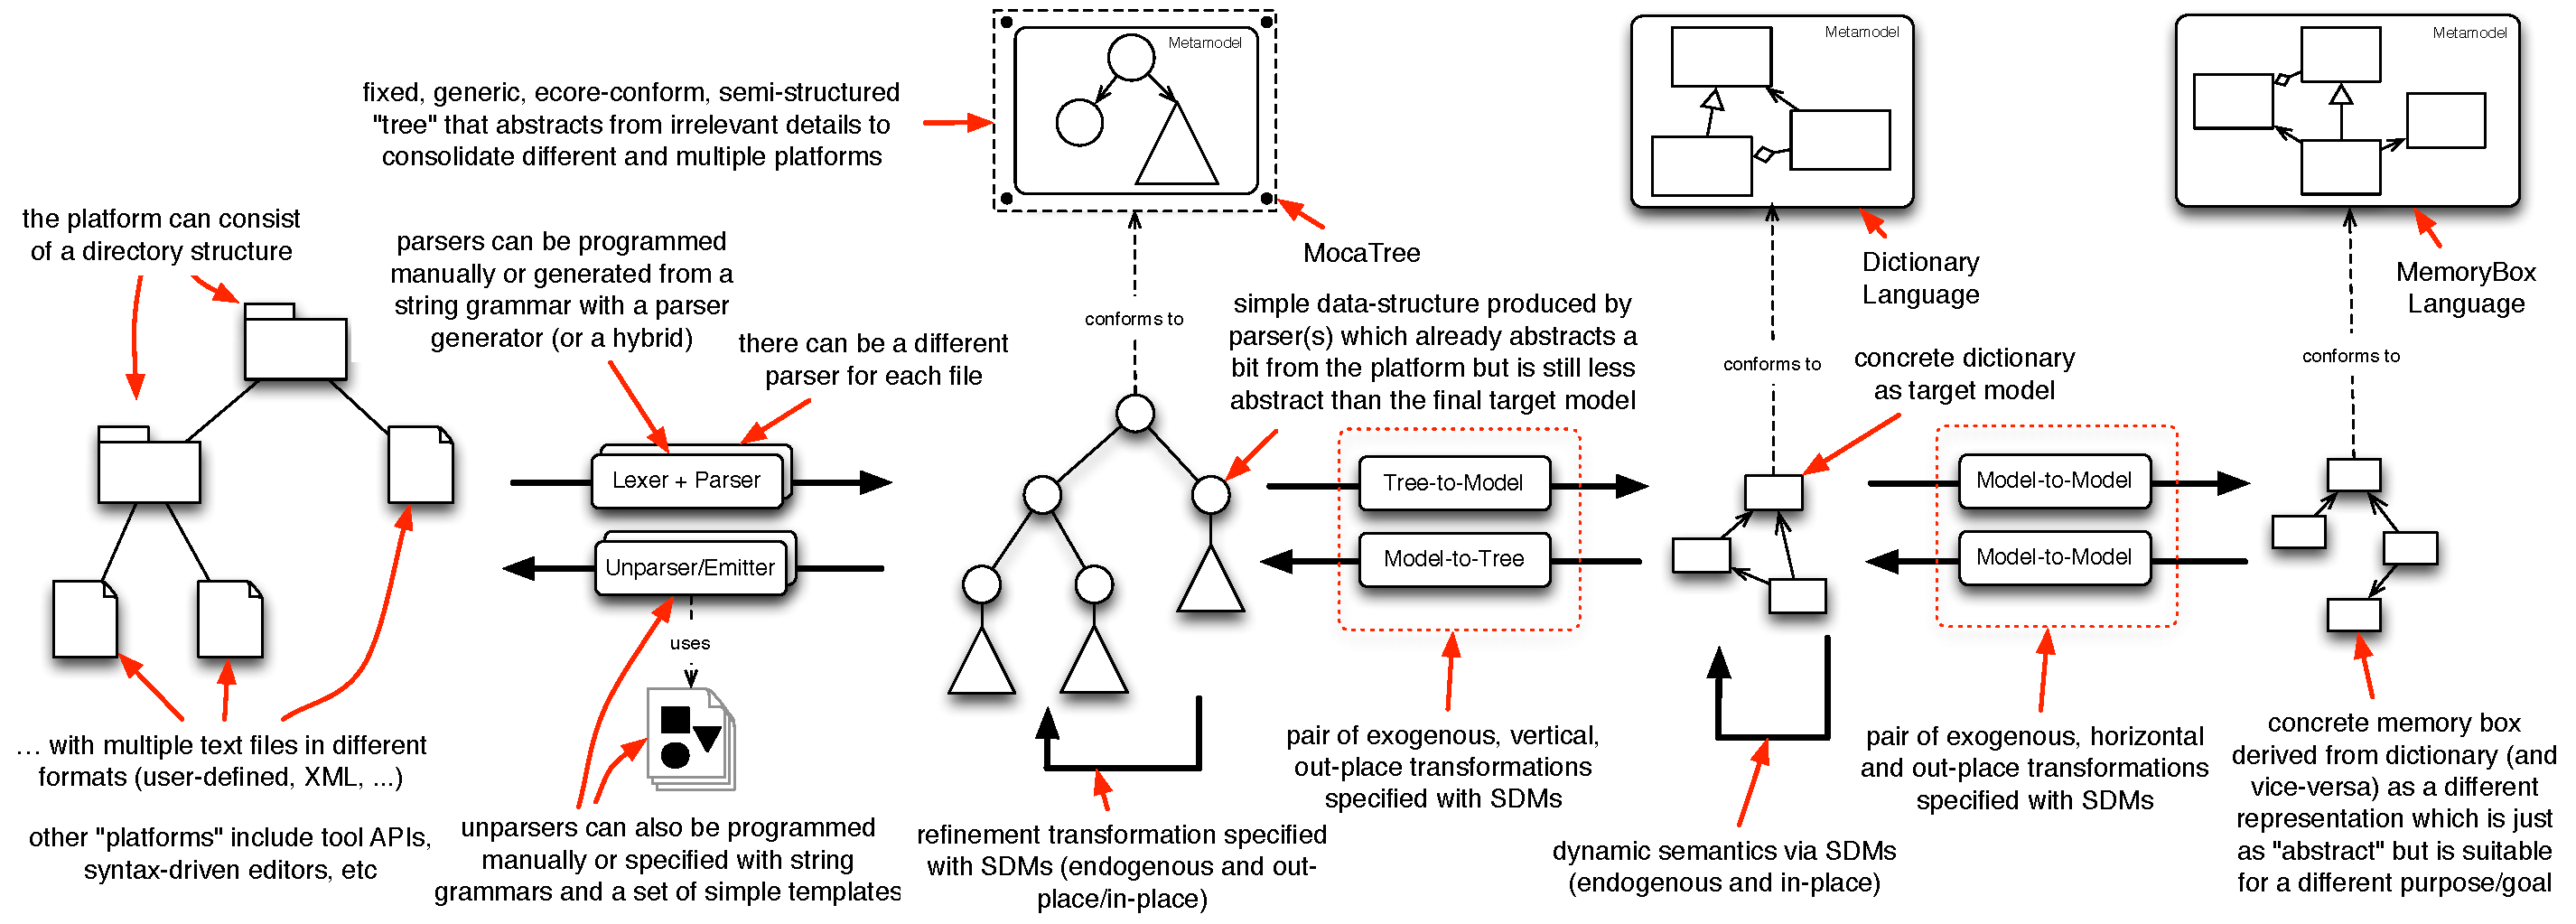
\includegraphics[angle=90, height=\textheight]{pics/moca/text-to-model}
%   \caption{Overview of model-to-text with the MOCA framework}
%   \label{fig:moca-overview}
% \end{center}
% \end{figure} 


% --- Getting both metamodels and parser set up
\newpage
\section{Setting up the workspace}
\genHeader

Nowadays, \emph{no one} writes a complex parser completely by hand. Although this is sometimes still necessary for syntactically challenging languages, most
parsers can be quickly whipped up using context-free \emph{string grammars}.\footnote{For simple cases, \emph{regular expressions} can also be used} These are
typically written in Extended Backus-Naur Form (EBNF)\define{EBNF}. ANTLR~\cite{ANTLR} is a tool that can generate a parser from this compact specification for
a host of target programming languages, including Java. Although ANTLR might not be the most efficient or powerful parser generator, it is open-source, well
documented and supported, and allows for a pragmatic and elegant fallback to Java when things get nasty and we have to resort to some dirty tricks to get our
job done.

A parser, of course, is based on whatever model it must work with. Given that we want to parse to and from a dictionary, we need to have the
\texttt{DictionaryLanguage} metamodel defined before starting. The dictionary is a relatively simple device, so you have three options to loading this project
into your workspace:

% Options
\begin{description}
% -- Metamodel Screenshots ---
\item[Option 1:] You can start a new metamodel project called \texttt{Dictionary} (Fig.~\ref{eclipse:startMetamodel}) and complete a
\texttt{DictionaryLanguage} package until it matches either Fig.~\ref{ea:dictLang} or Fig.~\ref{eclipse:dictLang}.\footnote{Review metamodel construction by
working through Part II: Ecore}

\begin{figure}[htbp]
\begin{center}
  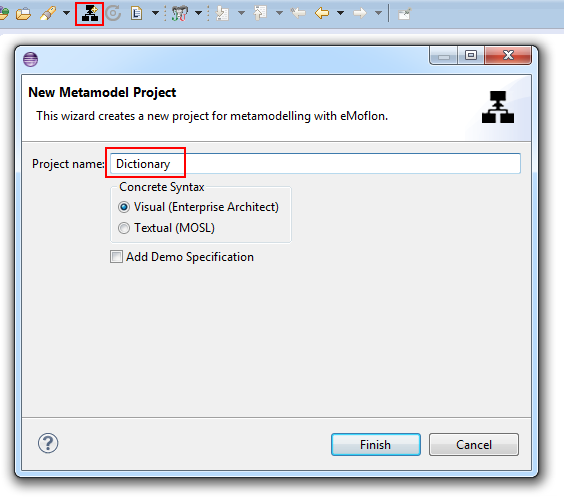
\includegraphics[width=0.65\textwidth]{eclipse_startDictionary}
  \caption{Begin parser project}
  \label{eclipse:startMetamodel}
\end{center}
\end{figure}

\newpage

\vspace*{1cm}

\begin{figure}[htb]
\begin{center}
  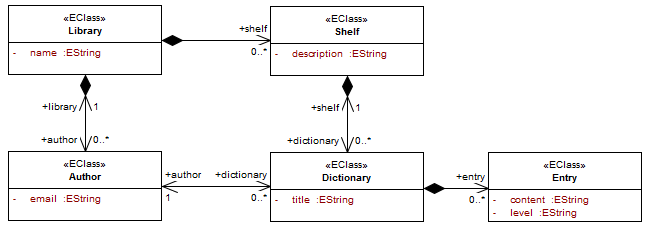
\includegraphics[width=\textwidth]{ea_dictionaryMetamodel}
  \caption{TCreate the package in \texttt{My Working Set} with an eMoflon Ecore diagram of the same name.}
  \label{ea:dictLang}
\end{center}
\end{figure}

\vspace{1cm}

\begin{figure}[htb]
\begin{center}
  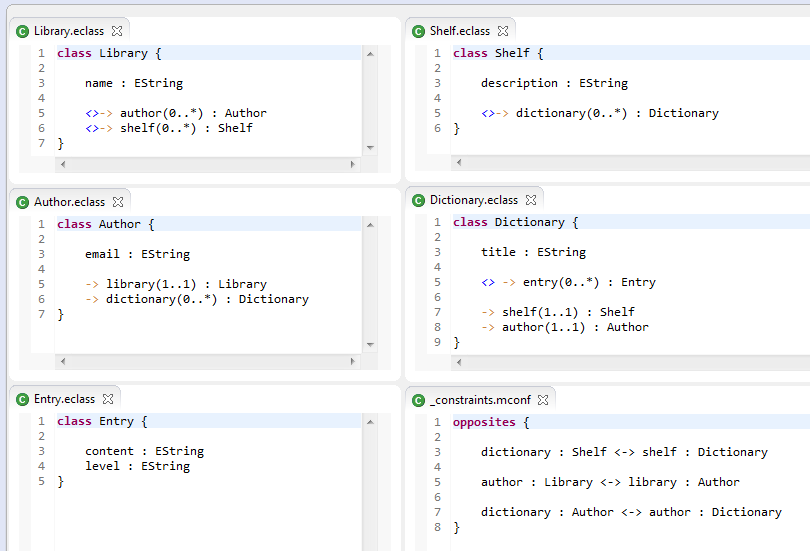
\includegraphics[width=0.8\textwidth]{eclipse_dictionaryMetamodel}
  \caption{\texttt{Dictionary} constructed in Eclipse \update}
  \label{eclipse:dictLang}
\end{center}
\end{figure}

\newpage

% -- Cheat Package(s)
\newpage
\item[Option 2:] You can download our cheat package and load \texttt{Dictionary} into your workspace using the Eclipse ``New" wizard
(Fig.~\ref{eclipse_cheatPackage}).

\vspace{0.5cm}

\begin{figure}[htbp]
\begin{center}
  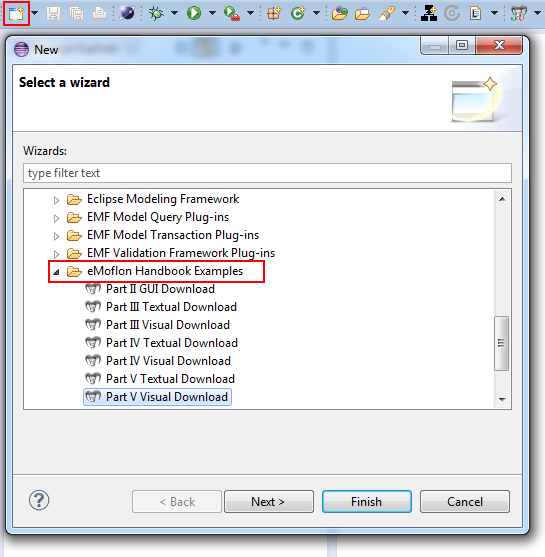
\includegraphics[width=0.65\textwidth]{eclipse_loadDictionaryProject}
  \caption{Load a \texttt{Dictionary} project into your workspace}
  \label{eclipse_cheatPackage}
\end{center}
\end{figure}

\item[$\blacktriangleright$] Pressing \texttt{Finish} will load either a MOSL directory or \texttt{DictionaryLanguage.eap} file into a working set, depending on
your syntax choice (Fig.~\ref{ea:cheatLoaded} or Fig.~\ref{eclipse:cheatLoaded}).

\begin{figure}[htbp]
   \centering
      \subfloat[comment 1 \update]{
        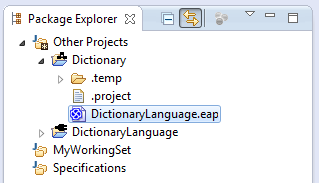
\includegraphics[width=0.45\textwidth]{eclipse_loadedCheatPackageVisual}
        \label{ea:cheatLoaded}
      }
      \subfloat[Bugger. Comment 2]{
        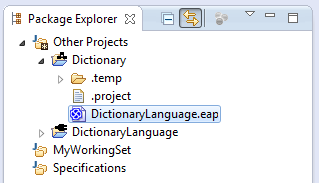
\includegraphics[width=0.45\textwidth]{eclipse_loadedCheatPackageVisual}
        \label{eclipse:cheatLoaded}
      }
      \caption{}
\end{figure}


\clearpage
% -- Export/Import ----
\item[Option 3:] You can simply use the same \texttt{Dictionary} you used in part IV by exporting it to a new project. Read Part IV, Section 2 for detailed
review on how to do this in either syntax.

\end{description} 
% -- End

\vspace{0.5cm}

This metamodel is one of two that we'll be using to specify the transformation. After all, as discussed in the introduction of Part IV, TGGs \emph{always}
require a source and target graph, and this will represent our target. 

We recommend inspecting \texttt{DictionaryLanguage} until you feel comfortable with what you'll be working with. As you'll be able to see, a \texttt{Library}
can contain an unlimited number of \texttt{Shelf} and \texttt{Author} elements. Both of these are also connected to a \texttt{Dictionary} container which can
hold an unlimited number of \texttt{Entry} objects.

Our source metamodel will be eMoflon's standard \texttt{MocaTree} language. It basically combines concepts from a filesystem (folders and files), XML concepts
(text-only nodes and attributes), and a general indexed containment hierarchy.\footnote{This is done with an index attribute, which can be used to demand a
certain \emph{order} of nodes in an SDM which are otherwise not guaranteed by default.} It models a generic directory structure with a \texttt{Folder} able to
connect to other \texttt{Folders}, and may contain an unlimited number of \texttt{File} elements. Its Jaca code is provided by the Eclipse plugin and
automatically added to the Java build path.  We'll go into more detail about this later, so let's skip ahead to the next task: initializing the TGG project that
will drive our model-to-text transformation.

\jumpDual{initialize vis}{initialize tex}

\newpage
\hypertarget{initialize vis}{}
\subsection{First steps}
\visHeader

\begin{itemize}

\item[$\blacktriangleright$] From your Eclipse workspace, open the \texttt{Dict\-ion\-ary.eap} file in Enterprise Architect (EA). The project browser should
closely resemble Fig.~\ref{ea:mocaTagged}. As you can see, the project is already populated with \texttt{MocaTree} and other built-in metamodels
in the \texttt{eMoflon Languages} working set.

\vspace{0.5cm}

\begin{figure}[htpb]
\begin{center}
  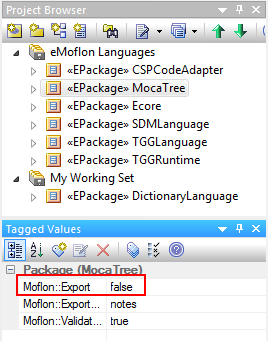
\includegraphics[width=0.4\textwidth]{ea_mocaTaggedValues}
  \caption{\texttt{MocaTree} is one of eMoflons' internal metamodels}
  \label{ea:mocaTagged}
\end{center}
\end{figure}

\end{itemize}

\vspace{-0.5cm}

If you inspect the tagged values\footnote{The ``Tagged Values'' window can be opened by going to ``View/Tagged Values'' or by hovering over the \texttt{Tagged
Values} tab immediately to the right of the project browser.} for these built-in languages, you'll notice that the \texttt{MocaTree} package has the
\texttt{Moflon::Export} value set to \texttt{false}. This ensures that the package is \emph{ignored} when exporting. As with all such standard metamodels (e.g.,
Ecore or our SDM metamodel) the \texttt{MocaTree} package in EA should be regarded as read-only, required only in the EA project so that SDMs/TGGs can refer to
the classes defined in the package.

\begin{itemize}

\item[$\blacktriangleright$] Despite \texttt{DictionaryLanguage} being contained in a different working set than \texttt{MocaTree}, the two
metamodels are contained within the same EA project (EAP) which means you are able to create a new TGG using them both. Add a new package to \texttt{My
Working Set} named \texttt{Dict\-ion\-ary\-Code\-Adap\-ter}.

\item[$\blacktriangleright$] Select the package and add a new TGG schema diagram as depicted in Fig.~\ref{ea:newTGGDiagram}. In the next dialogue window,
set the source project as \texttt{MocaTree}, and the target project as \texttt{Dict\-ion\-ary\-Lang\-uage}.

\begin{figure}[h!]
\begin{center}
  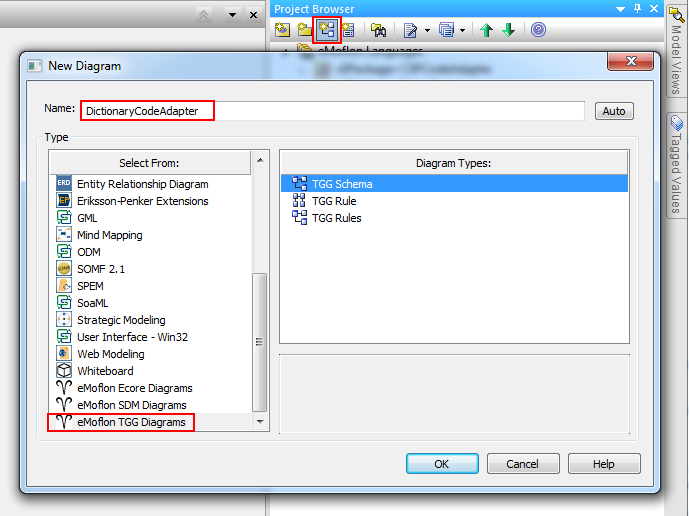
\includegraphics[width=0.9\textwidth]{ea_adapterTGGDiagram}
  \caption{Create a new TGG schema diagram}
  \label{ea:newTGGDiagram}
\end{center}
\end{figure}

\item[$\blacktriangleright$] For the moment, add a single correspondence type to the new diagram now active in the editor (the TGG \texttt{schema}) between
\texttt{Folder} and \texttt{Library}. Remember, you can get the classes by drag-and-dropping each element into the diagram, then quick-creating a new
\texttt{TGG Correspondence Type} between them.\footnote{For details on the correspondence metamodel and how to create types, refer to Part IV, Section 3.} Your diagram
should come to resemble Fig.~\ref{ea:firstCorrType}.

\vspace{0.5cm}

\begin{figure}[htpb]
\begin{center}
  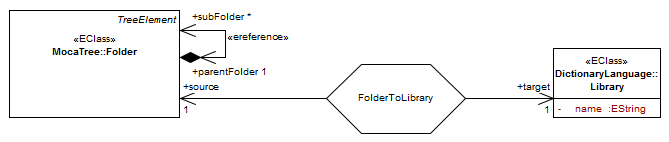
\includegraphics[width=\textwidth]{ea_firstAdapterCorrespondence}
  \caption{The first correspondence type for the transformation}
  \label{ea:firstCorrType}
\end{center}
\end{figure}

\newpage

\item[$\blacktriangleright$] Your complete project browser should now resemble Fig.~\ref{ea:TGGProjBrow}, where \texttt{Dict\-ion\-ary\-Code\-Adap\-ter} is now
explicitly listed as a \texttt{TGGSchemaPackage}.

\vspace{0.5cm}

\begin{figure}[htpb]
\begin{center}
  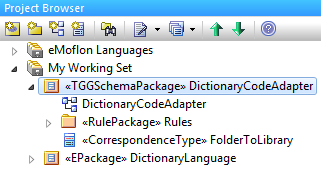
\includegraphics[width=0.5\textwidth]{ea_TGGProjectBrowser}
  \caption{A fully prepared TGG project}
  \label{ea:TGGProjBrow}
\end{center}
\end{figure}

\item[$\blacktriangleright$] Validate and export your file via the eMoflon control panel,\footnote{Activate via ``Extensions/Add-in Windows''} then switch
back to Eclipse and refresh the package explorer. A new \texttt{Dict\-ion\-ary\-Code\-Adap\-ter} project should appear in \texttt{My Working Set}.

\jumpSingle{subSec:setupParser}

\end{itemize}


\newpage
\hypertarget{M2TSettingUp tex}{}
\subsection{Initializing the project}
\texHeader

{\bf SELF:: update download so it includes a constraint file for \texttt{Dictionary}}
\begin{figure}[htbp]
\begin{center}
  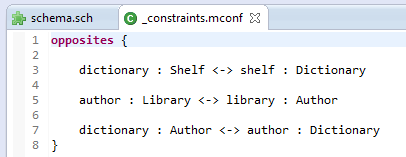
\includegraphics[width=0.7\textwidth]{eclipse_DOWNLOADUPDATE}
  \caption{SELF SELF}
\end{center}
\end{figure}

\begin{enumerate}

\item[$\blacktriangleright$] Your expanded \texttt{DictionaryLanguage} metamodel MOSL structure should resemble FIG. (starting point) You'll notice that it is
accessing the \emph{Moca} framework by importing the \texttt{MocaTree} in \texttt{\_imports.mconf}. (Explain, no screenshot?)

\item[$\blacktriangleright$] Right click on \texttt{MyWorkingSet} folder and create a new TGG. source: MocaTree. Target: DictionaryLanguage. FIG

\begin{figure}[htbp]
\begin{center}
  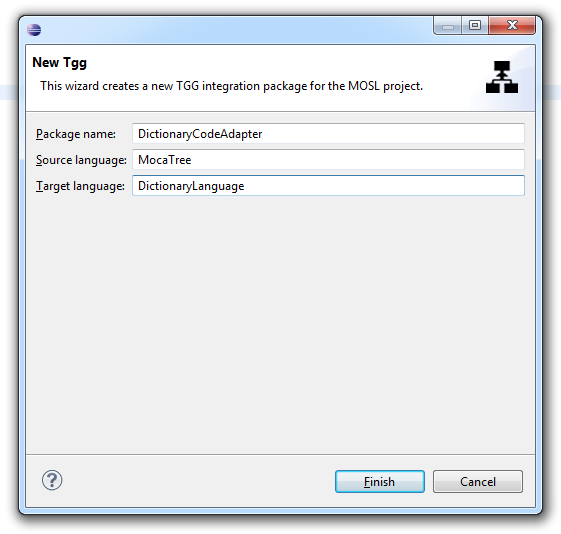
\includegraphics[width=0.9\textwidth]{eclipse_dictionaryCodeAdapterTGGProject}
  \caption{create tgg}
  \label{eclipse:newTGGProject}
\end{center}
\end{figure}


\item[$\blacktriangleright$] Before saving and building, initialize the correct generated code type by establishing the schema below (default is..)

\begin{figure}[htbp]
\begin{center}
  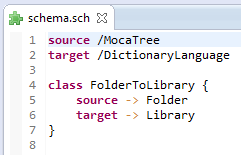
\includegraphics[width=0.5\textwidth]{eclipse_schemaStart}
  \caption{first rule}
  \label{eclipse:firstSchema}
\end{center}
\end{figure}

\item[$\blacktriangleright$] Save and build your project! Confirm a generated project was created in the \texttt{MyWorkingSet} node, and carry on!

\end{enumerate}


\newpage
\hypertarget{subSec:setupParser}{}
\subsection{Setting up the Parser}
\genHeader

\begin{itemize}

\item[$\blacktriangleright$] It should now resemble Fig.~\ref{eclipse:generatedAdapter}. Be sure to take a look at the \texttt{Moflon} and \texttt{Moca} library
nodes that reference jars for all required dependencies.

\begin{figure}[htpb]
\begin{center}
  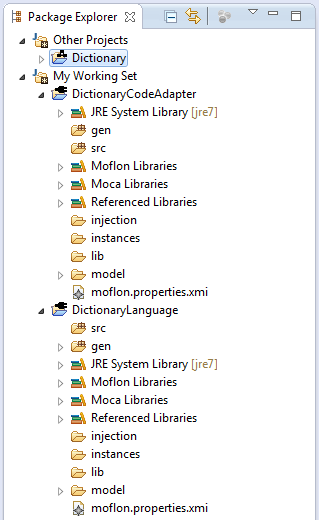
\includegraphics[width=0.4\textwidth]{eclipse_generatedAdapter}
  \caption{figureCaption}
  \label{eclipse:generatedAdapter}
\end{center}
\end{figure}

\item[$\blacktriangleright$] Right-click on \texttt{DictionaryCodeAdapter} and navigate to ``eMolfon/ Add Parser/Unparser'' (Fig~\ref{eclipse:contextParser}).

\begin{figure}[htpb]
\begin{center}
  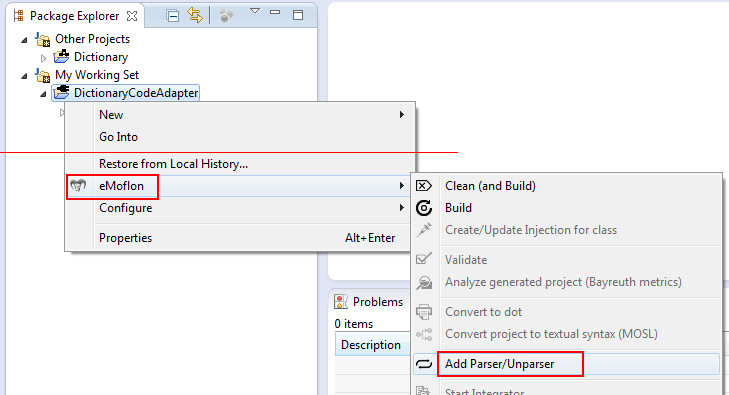
\includegraphics[width=0.9\textwidth]{eclipse_contextAddParserUnparser}
  \caption{figureCaption}
  \label{eclipse:contextParser}
\end{center}
\end{figure}

\item[$\blacktriangleright$] In the wizard dialogue (Fig~\ref{eclipse:wizardParser}), enter ``dictionary'' as the \texttt{File extension}, and make sure
the boxes \texttt{Create Parser} and \texttt{Create Unparser} with \texttt{ANTLR} are chosen as corresponding technology in both cases. Click \texttt{Finish} to
close.

\begin{figure}[htpb]
\begin{center}
  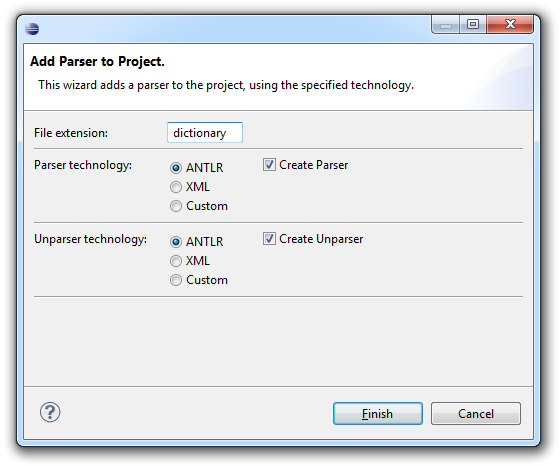
\includegraphics[width=0.8\textwidth]{eclipse_wizardParser}
  \caption{figureCaption}
  \label{eclipse:wizardParser}
\end{center}
\end{figure}

If everything has been installed and set up properly, parser and unparser stubs should be generated and \texttt{ANTLR} should automatically build the
corresponding Java code as depicted in Fig.~\ref{eclipse:generatedParser}.

\begin{figure}[htpb]
\begin{center}
  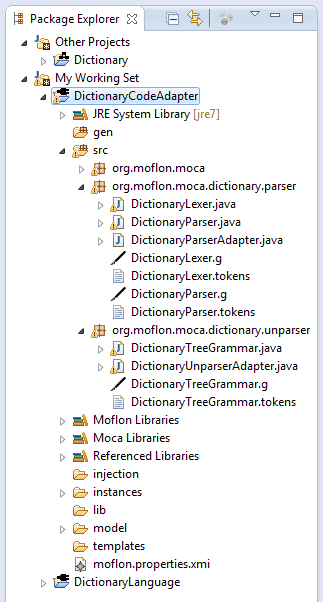
\includegraphics[width=0.4\textwidth]{eclipse_generatedParser}
  \caption{figureCaption}
  \label{eclipse:generatedParser}
\end{center}
\end{figure}

\end{itemize}


 
% --- First Direction
\newpage
\section{Text-to-tree transformation}
\genHeader

Now that our workspace is successfully prepared, let's discuss how the transformation will proceed. For reference, Fig.~\ref{fig:moca-4-Tokens} depicts a small
sample of the textual syntax that will specify a dictionary instance. As we shall see in a moment, the libraries and shelves containing each dictionary correspond to a folder structure, while the
contents for a single dictionary are specified in a file.

\begin{figure}[!htbp]
\begin{center}
 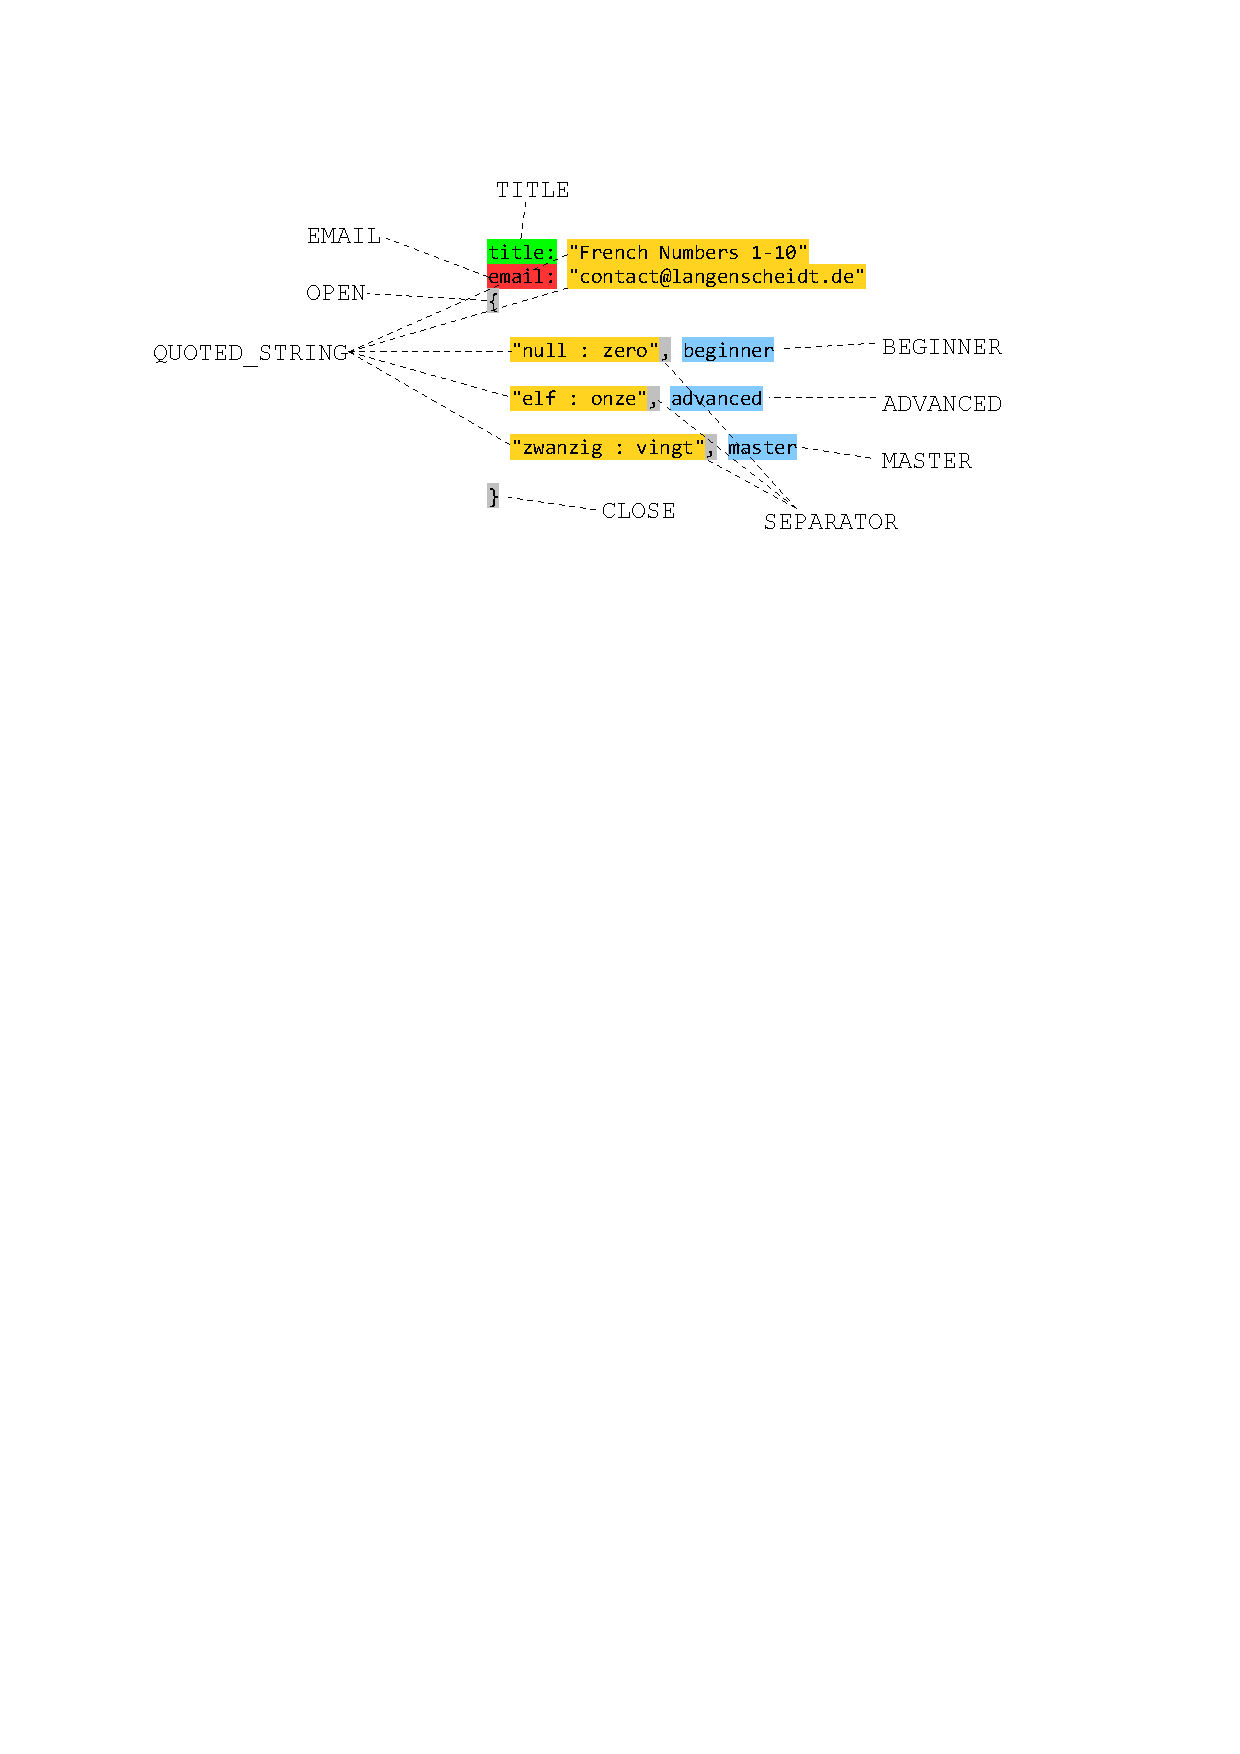
\includegraphics[width=0.7\textwidth]{4-tokens}
  \caption{Identified tokens in a dictionary file}
  \label{fig:moca-4-Tokens}
\end{center}
\end{figure}

On the way to an instance model of our dictionary metamodel, the very first step is to create nice \emph{chunks} of characters. This step is called
\emph{lexing} and it simplifies the comprehension of the complete text. Interestingly, human beings actually comprehend text in a similar manner; one
recognizes whole words without ``seeing'' every individual character. This is the reason why you can siltl raed tihs sneentce alsomt eforftlsesly. A lexer
recognizes these chunks or \emph{tokens} and passes them on as a token stream to the \emph{parser} that does the actual work of recognizing complex
hierarchical and recursive structures.
   
To recognize the tokens as indicated in Fig.~\ref{fig:moca-4-Tokens}, \texttt{ANTLR} can automatically generate a lexer in Java from a compact specification.
This is actually a DSL for lexing and is explained in detail in \cite{ANTLR}. If you are unfamiliar with EBNF, and feel you may have problems understanding
the lexer grammar, we suggest going through the documentation on \url{www.antlr.org}, or reading the relevant chapters in \cite{ANTLR}. Otherwise, let's
complete the \emph{lexer} and \emph{parser} grammars that will handle our project instances.

\begin{itemize}
  
\item[$\blacktriangleright$] Navigate to ``Diction\-ary\-Code\-Adap\-ter/src/org.moflon.moca.dict\-ion\-ary\-.pars\-er" and edit \texttt{DictionaryLexer.g}
until it matches Fig.~\ref{eclipse:dictionaryLexer}. 


\newpage

\begin{figure}[!htbp]
\begin{center}
  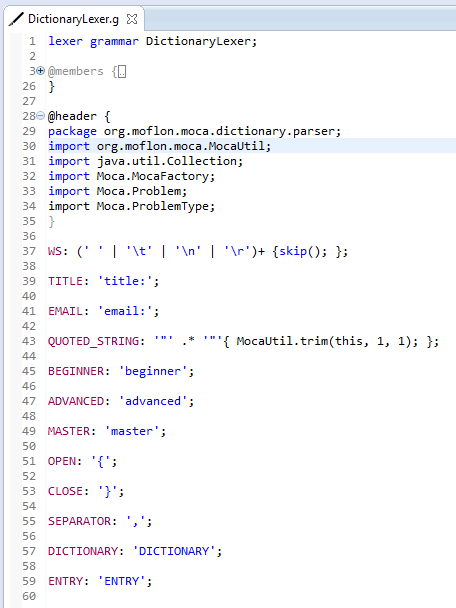
\includegraphics[width=0.7\textwidth]{eclipse_dictionaryLexer}
  \caption{Lexer grammar}
  \label{eclipse:dictionaryLexer}
\end{center}
\end{figure}

\item[$\blacktriangleright$] Don't forget to add \texttt{import org.moflon.moca.MocaUtil} to \texttt{@header}. Be vigilant to avoid any typos and mistakes!

\vspace{0.5cm}

\item[$\blacktriangleright$] Save to compile the file, and ensure no errors persist before proceeding.

\end{itemize}

\vspace{0.25cm}

To briefly explain the two complicated-looking rules, note that the \texttt{WS} rule simply ignores white space. The \texttt{`skip()'} statement throws away the
tokens matched as white space each time they're found in a stream. Similarly, \texttt{QUOTED\_STRING} calls \texttt{`MocaUtil.trim(\ldots)'}, which trims a
recognized token by removing the specified number of characters at its beginning and end. In this case, the token is everything between the `\texttt{''}'
characters, as indicated by the \texttt{`.*'} symbol.

\newpage

Now let's establish a parser to form a file's stream of tokens (as created by the lexer) into a \emph{tree}. In this context, a tree is an acyclic,
hierarchical, recursive structure as depicted in Fig.~\ref{fig:dictLexer}. Depending on what the tree is to be used for, it can be organized differently
using extra \emph{structural} nodes such as \texttt{DICTIONARY} or \texttt{ENTRY} which were not present in the textual syntax. These can be used to give
additional semantics to the tree.

\vspace{0.5cm}

\begin{figure}[htp]
\begin{center}
 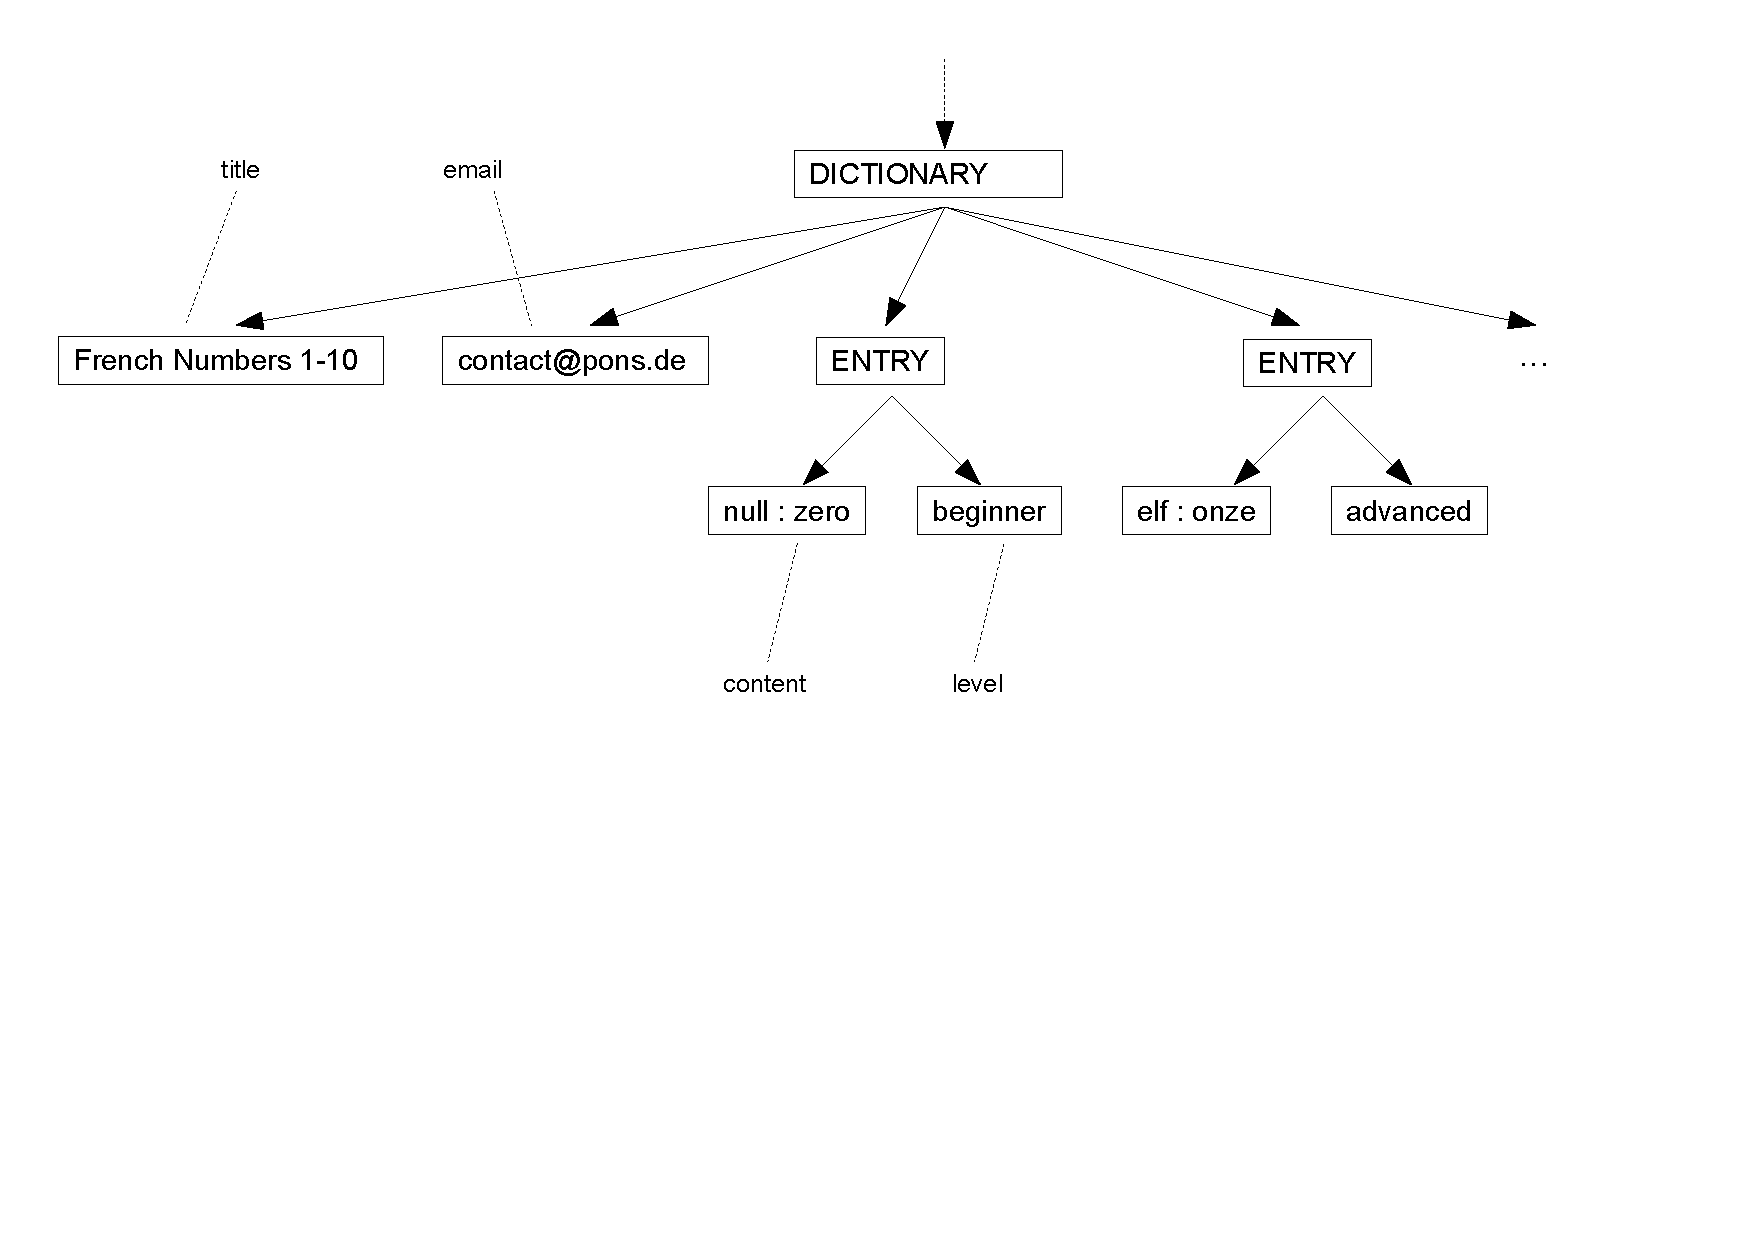
\includegraphics[width=\textwidth]{5-tree}
  \caption{Abstract Syntax Tree (AST) of an input token stream}
  \label{fig:dictLexer}
\end{center}
\end{figure}

\begin{itemize}

\item[$\blacktriangleright$] From the same package, open and edit \texttt{DictionaryParser.g} until it matches Fig.~\ref{eclipse:dictParser}. As with the lexer,
avoid any mistakes, and ensure it compiles before proceeding.

\end{itemize}

\begin{figure}[!htbp]
\begin{center}
 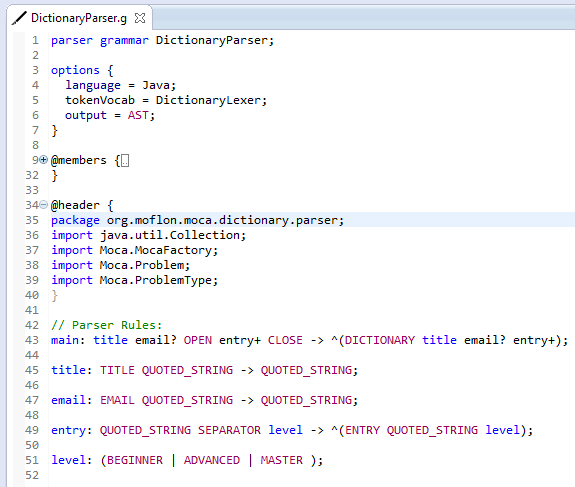
\includegraphics[width=0.9\textwidth]{eclipse_dictionaryParser}
  \caption{Parser grammar}
  \label{eclipse:dictParser}
\end{center}
\end{figure}

You'll notice that the parser grammar is extremely similar to the lexer grammar, save for some \emph{parser actions} following the \texttt{`->'} symbol. These
actions control the construction of the resulting tree. Using this simple tree language, one can (1) abstract from tokens such as \texttt{`\{'} or
\texttt{`\}'}, which are just \emph{syntactical noise}\footnote{Irrelevant content for our model} and (2) enrich the tree with structural nodes such as
\texttt{ENTRY}, which add explicit structure to the tree. Refer to \cite{ANTLR} and online resources for detailed explanations on the syntax and semantics of
the parser grammar supported by \texttt{ANTLR}.

\newpage

\begin{itemize}

\item[$\blacktriangleright$] Before taking our lexer and parser for a spin, navigate to ``src\-/org\-.mof\-lon\-.tie" and open
\texttt{DictionaryCodeAdapterTrafo.java}. We need to update the file so that it will work with our specific project, so add the highlighted areas in
Fig.~\ref{eclipse:defaultTGGMain} to the file.

\vspace{0.5cm}

\begin{figure}[!htbp]
\begin{center}
 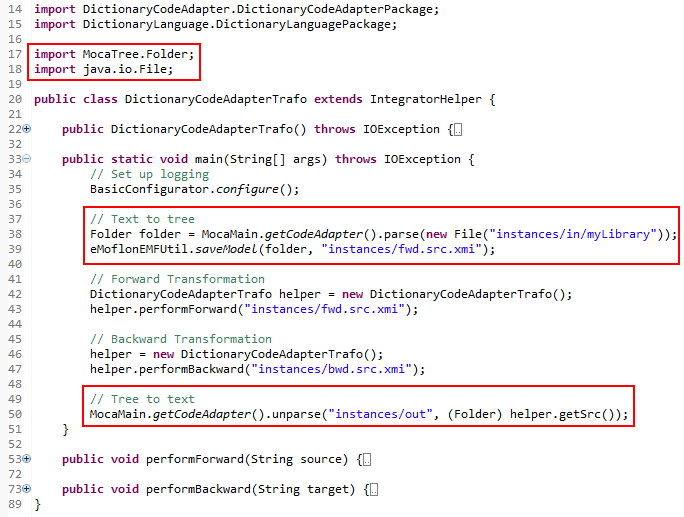
\includegraphics[width=\textwidth]{eclipse_editTrafo}
  \caption{Edit \texttt{DictionaryCodeAdapterTrafo} to run the transformation}
  \label{eclipse:defaultTGGMain}
\end{center}
\end{figure}

\end{itemize}

You can see that this main method is essentially the driver for a complete transformation, executing four stages for a forward and backward transform. In a
nutshell, each folder in ``instances/in/myLibrary'' is taken as the root of a tree, and their folder and file structures will be reflected as a hierarchy of
(children) nodes in the tree. For each file, the framework will search for a registered parser that is responsible for the particular file, pass the content
onto the parser, then plug in the tree generated from the parser as a single subtree of the corresponding file node in the overall tree.

In this example, the framework uses our parser on \texttt{.dictionary} files, the file extension we specified when creating the lexer and parser stubs
(Fig.~\ref{eclipse:generatedParser}). Of course, this method (in the generated \texttt{parserAdapter}) can be overridden to register e.g., multiple
file extensions, or peek into the actual file content and base its parsing decision on what it finds.

\begin{itemize}

\item[$\blacktriangleright$] To prepare some input for the framework, navigate to ``Dict\-ion\-ar\-y\-Code\-Adap\-ter\-/in\-stan\-ces\-/in'' and create the
filesystem depicted in \\ Fig.~\ref{eclipse:textDirectory}. 

\begin{figure}[htp]
\begin{center}
  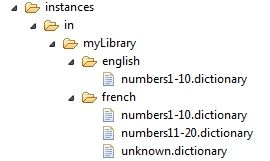
\includegraphics[width=0.5\textwidth]{inputData}
  \caption{Input directory structure}
  \label{eclipse:textDirectory}
\end{center}
\end{figure}

\item[$\blacktriangleright$] Complete each of the four \texttt{.dictionary} files with the contents in Table~\ref{moca-inputdata}.\footnote{If you copy and
paste this data, be careful as your .pdf reader may add some invisible characters to the file that ANTLR will not detect and ignore as white space.} 
Be vigilant to ensure there are no mistakes with symbols such as colons or commas!

\end{itemize}

As you can see, the input folder is structured as a single library, \texttt{myLibrary}, and split into two languages, english and french, each containing
some dictionaries. Reviewing Fig.~\ref{eclipse:dictParser}, you can see that the structure of these files conforms to the parser's \texttt{main} rule: it
first lists the dictionary's \texttt{title}, may or may not contain an \texttt{author}, and contains all \texttt{entry} elements between a pair of \texttt{OPEN}
and \texttt{CLOSE} brackets.

\newpage
\begin{table}

\begin{tabular}{p{6cm} p{6cm} }
\footnotesize
\textbf{english/numbers1-10.dictionary:}
\begin{verbatim}
title: "numbers1-10"
email: "contact@langenscheidt.de"	
{
  "null : zero", beginner
  "eins : one", beginner
  "zwei : two", beginner
  "drei : three", beginner
  "vier : four", beginner
  "fuenf : five", beginner
  "sechs : six", beginner
  "sieben : seven", beginner
  "acht : eight", beginner
  "neun : nine", beginner
  "zehn : ten", beginner 
}
\end{verbatim} 

\vspace{0.5cm}

\footnotesize
\textbf{french/numbers11-20.dictionary:}
\begin{verbatim}
title: "numbers11-20"
email: "contact@pons.de"	
{
  "elf : onze", advanced
  "zwoelf : douze", advanced
  "dreizehn : treize", advanced
  "vierzehn : quatorze", advanced
  "fuenfzehn : quinze", advanced
  "sechzehn : seize", master
  "siebzehn : dix-sept", master
  "achtzehn : dix-huit", master
  "neunzehn : dix-neuf", master
  "zwanzig : vingt", master
}
\end{verbatim}
&

\footnotesize
\textbf{french/numbers1-10.dictionary:}
\begin{verbatim}   
title: "numbers1-10"
email: "contact@pons.de"	
{
  "null : zero", beginner
  "eins : un/une", beginner
  "zwei : deux", beginner
  "drei : trois", beginner
  "vier : quatre", beginner
  "fuenf : cinq", beginner
  "sechs : six", beginner
  "sieben : sept", beginner
  "acht : huit", beginner
  "neun : neuf", beginner
  "zehn : dix", beginner 
}
\end{verbatim}

\vspace{0.5cm}

\footnotesize
\textbf{french/unknown.dictionary:}
\begin{verbatim}
title: "unknown"
{
	"unbekannt : unknown", beginner
}
\end{verbatim}
  \\
\end{tabular}   
\caption{Four input \texttt{.dictionary} files}
\label{moca-inputdata}

\end{table}
\clearpage

\begin{itemize} 

\item[$\blacktriangleright$] Once you have saved each file, right click on \texttt{Dict\-ion\-ar\-y\-Code\-Ad\-ap\-ter\-Traf\-o.\-java} and navigate to ``Run
As/Java Application'' to run the transformation. Don't worry about the error messages -- they're related to the unparser which we haven't implemented yet; You
should have received at least one success message indicating your transformation worked.

\item[$\blacktriangleright$] Refresh the \texttt{instances} folder. Despite being (mostly) unimplemented, the transformation still partly completed, generating
several files in the process (Fig.~\ref{eclipse:postParse}).

\vspace{0.5cm}

\begin{figure}[!htbp]
\begin{center}
 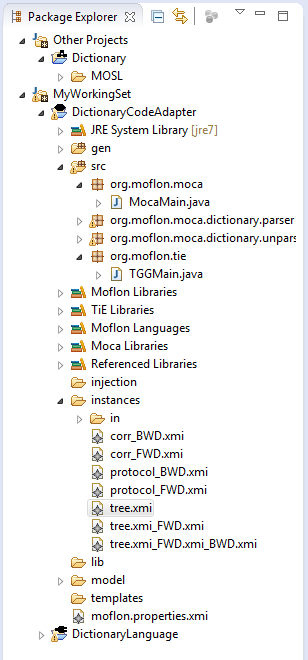
\includegraphics[width=0.5\textwidth]{eclipse_explorerPostGeneration}
  \caption{Result of the first TGG execution}
  \label{eclipse:postParse}
\end{center}
\end{figure} 

\end{itemize}

Let's go over what each of these files are. First, \texttt{fwd.src.xmi} is the direct result of the \texttt{my\-Lib\-rary} filesystem input, which was parsed
into a \texttt{MocaTree} instance by our ANTLR parser. 

While the parser is the only implemented piece of our transformation, TGGMain still used \texttt{fwd.src.xmi} in a forward transform, producing
the correspondence model \texttt{fwd.corr.xmi} (paired with \texttt{fwd.protocol.xmi}), and the (currently empty) \texttt{Dictionary} target result,
\texttt{fwd.trg.xmi}.

\clearpage

%The TGG also executed in the inverse direction; \texttt{tree.xmi\_FWD.xmi} was used in the backwards direction, producing \texttt{corrBWD.xmi} (with
%\texttt{proto\-col\-\_BWD\-.xmi}) and \texttt{tree.xmi\_FWD.xmi\_BWD.xmi}. 

\begin{itemize}

\item[$\blacktriangleright$] Open \texttt{fwd.src.xmi} and compare the contents to Fig.~\ref{eclipse:treeResult}. Reflect on the directory-type structure of the
tree, where each \texttt{File} and its contents appear as \texttt{Node}s.\footnote{Refer to Fig~\ref{mocaTreeMetamodel} for the metamodel of this structure}
This file is important to understand -- The filesystem was transformed into a corresponding hierarchy of \texttt{Folders} and \texttt{Files}. The actual
\emph{text} content of each file is then transformed to a subtree using a registered, suitable parser. The resulting subtree from the parser is then connected
to the existing tree by setting its \texttt{DICTIONARY} root as the single child node of a \texttt{File}.

\end{itemize}

\vspace{0.5cm}

\begin{figure}[!htbp]
\begin{center}
 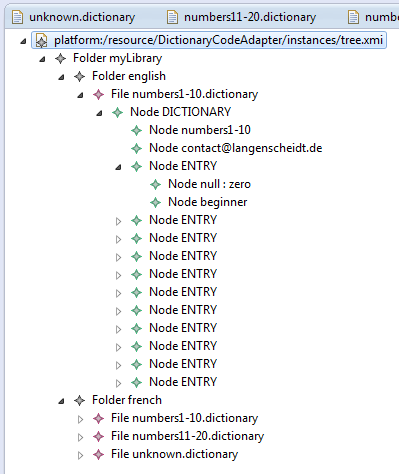
\includegraphics[width=0.6\textwidth]{eclipse_textParsingGeneration}
  \caption{A \texttt{MocaTree} created by the framework using our parser}
  \label{eclipse:treeResult}
\end{center}
\end{figure}

If everything executed without errors, well done! Let's continue with the transformation to a \texttt{Dictionary} instance by specifiying some
TGG rules.


% -- Second Direction 
\newpage
\section{Tree-to-model transformation with TGGs}
\genHeader

Our goal in this section is to break down the \texttt{MocaTree} to \texttt{Dictionary} transformation into smaller, modular steps. More precisely, we
want separate rules for transforming a \texttt{Folder} into its appropriate container element (i.e., \texttt{Library} or \texttt{Shelf}), then individual rules
to handle whatever \texttt{File} and \texttt{Node} elements they contain.

\vspace{0.5cm}

Let's briefly look at the models we'll be working with. We start with Fig.~\ref{eclipse:treeStart},\footnote{You can view this model in your Eclipse editor by
placing the contents of \texttt{fwd.src.xmi} into eMoflon's Graph Viewer, as
introduced in Part II, Section 4.} where our root input folder, \texttt{myLibrary}, contains two subfolders with at least one dictionary \texttt{File} each. Each dictionary has one equivalent dictionary root \texttt{Node} with at least two
children representing the title and first \texttt{ENTRY}, along with an unknown number of additional nodes. Of the remaining nodes, there may be one that stores
the dictionary author's contact information. All the rest will be \texttt{ENTRY} nodes with two children representing its content and level information.

\vspace{1cm}

\begin{figure}[htbp]
\hspace{-1.5cm}
 	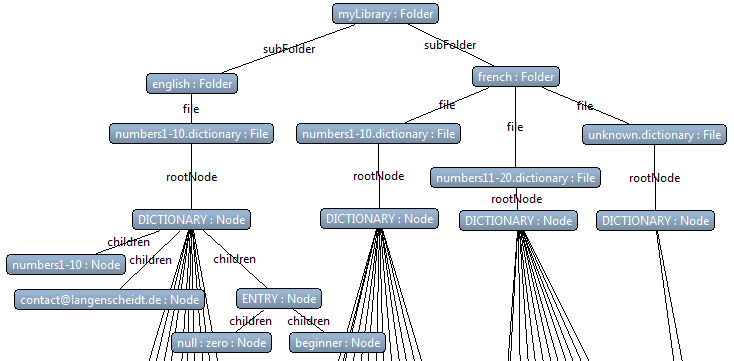
\includegraphics[width=1.2\textwidth]{eclipse_TreeStartMetamodel}
 	\caption{The \texttt{MocaTree} model of our input directory}
 	\label{eclipse:treeStart}
\end{figure}

\newpage

Our transformation intends to finish with a \texttt{Dictionary} model resembling
Fig.~\ref{eclipse:dictionaryStart}, where the root \texttt{myLibrary} has four children, one for each shelf and author. These elements will likely pair up, sharing a child \texttt{Dictionary} element containing an unknown number
of entries.

\vspace{1cm}

\begin{figure}[htbp]
\hspace{-1.5cm}
    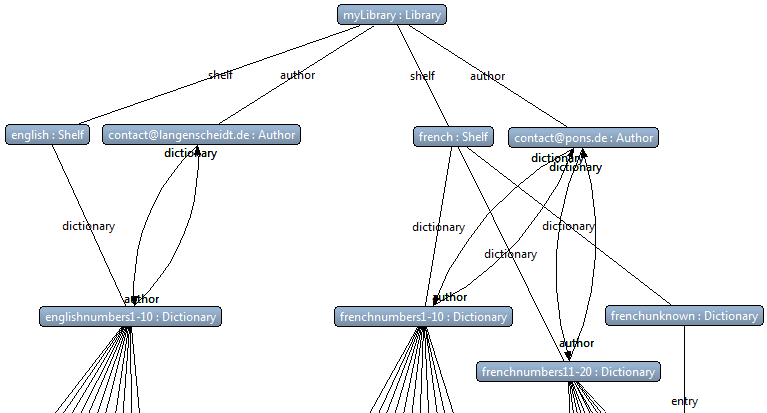
\includegraphics[width=1.2\textwidth]{eclipse_DictionaryResultMetamodel}
 	\caption{The final \texttt{Dictionary} target model}
 	\label{eclipse:dictionaryStart}
\end{figure}

\vspace{1cm}

As you can see, it's important to keep in mind the flexibility that the rules for this transformation will require. While our example model is small
enough to count the number of entries our rules will need to account for, future models may of course vary. Just like SDM patterns, it's key to avoid
situation-specific TGG rules.

\newpage
\hypertarget{treeToModel vis}{}
\subsection{The visual transformation rules}
\visHeader

\begin{itemize}

\item[$\blacktriangleright$] Expand the \texttt{<<Rules Package>>} node in EA and open the \texttt{Rules} diagram. Create a new rule named
\texttt{FolderToLibraryRule}, double-clicking the new element to open its diagram. Complete the rule as depicted in Fig.~\ref{ea:FolderIntoLibrary_Complete}.
Remember -- we established that first correspondence type when creating the TGG schema in Section 1.

\vspace{0.5cm}

\begin{figure}[htbp]
\begin{center}
  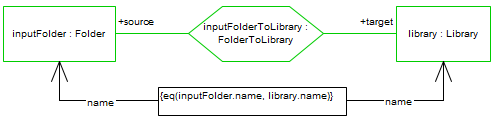
\includegraphics[width=0.8\textwidth]{ea_FolderToLibraryRule}
  \caption{completed folder into library}
  \label{ea:FolderIntoLibrary_Complete}
\end{center}
\end{figure}

\item[$\blacktriangleright$] We're able to use this entire rule as black context for the next rule in order to handle the creation of shelves. Select
\texttt{inputFolder, inputFolderToLibrary,} and \texttt{library}, then use the eMoflon control panel to \texttt{derive} a new rule. Name this \texttt{ForAllShelfRule}.

\item[$\blacktriangleright$] This will open a new diagram with three black objects, representing the context. This rule is remarkably similar to
\texttt{FolderToLibraryRule}, except it will need two green links connecting the new elements to their respective container. Complete \texttt{ForAllShelfRule}
as depicted in Fig.~\ref{ea:ForAllShelves_Complete}. You'll need to create a new correspondence type, \texttt{FolderToShelf} in either the schema (as we did
for \texttt{FolderToLibrary}) or by selecting \texttt{Create new Link} in the dialogue that appears from quick-linking between \texttt{shelfFolder} and
\texttt{shelf}.

\vspace{0.5cm}

\begin{figure}[htbp]
\begin{center}
  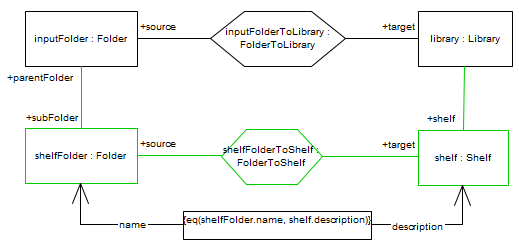
\includegraphics[width=0.8\textwidth]{ea_ForAllShelfRule}
  \caption{completed ForAllShelves}
  \label{ea:ForAllShelves_Complete}
\end{center}
\end{figure}

\newpage

\item[$\blacktriangleright$] Now we're able to handle the dictionary \texttt{File} elements. Ananlogously to how you began the previous rule, select
\texttt{shelfFolder}, \texttt{FolderToShelf}, and \texttt{shelf}, and derive \texttt{NodeToDictionaryRule}.

\item[$\blacktriangleright$] Build it as shown in Fig-~\ref{ea:NodeToDictionary_Complete}. As you can see, this rule creates a consistency between
\texttt{dictionaryNode} and the \texttt{dictionary} instance, and only handles the first \texttt{titleNode} in the tree structure. Nearly every element is
involved in order to correctly set the \texttt{dictionary} and \texttt{dictionaryFile} names in two different constraints!

\begin{figure}[htbp]
\begin{center}
  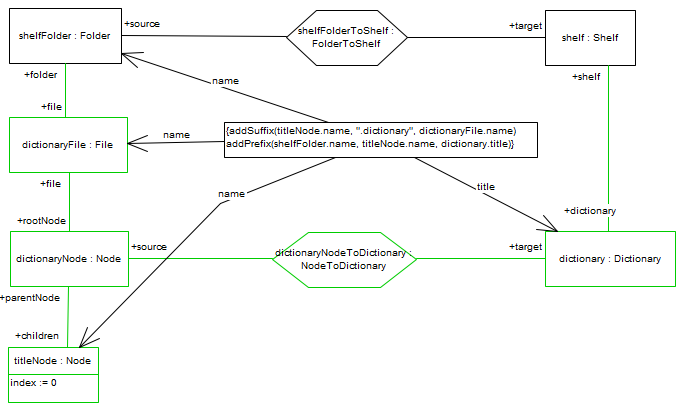
\includegraphics[width=\textwidth]{ea_NodeToDictionaryRule}
  \caption{completed NodeToDictionary}
  \label{ea:NodeToDictionary_Complete}
\end{center}
\end{figure}

\item[$\blacktriangleright$] Please note that the \texttt{index} \emph{attribute constraint} is required in order to ensure that the node with the title
information is correctly matched. We could have also included a \texttt{node} to handle the author, a third, fourth, or even tenth \texttt{node} connected to
\texttt{DictionaryNode}, but that would mean the pattern absolutely has to match to an author and ten elements, which may not always exist. Instead, we'll
create separate rules for each of these types which can be called as many times as necessary.

\item[$\blacktriangleright$] Let's handle the \texttt{entry} elements first. Create and complete \texttt{ForAllEntryRule} and depicted in
Fig.~\ref{ea:ForAllEntry_Complete}. We needed to match both a \texttt{contentNode} and \texttt{indexNode} to each \texttt{entryNode}, bound by their
\texttt{index} values in order to ensure the correct EString attributes were set to an \texttt{entry}'s \texttt{content} and \texttt{level} values.

\begin{figure}[htbp]
\begin{center}
  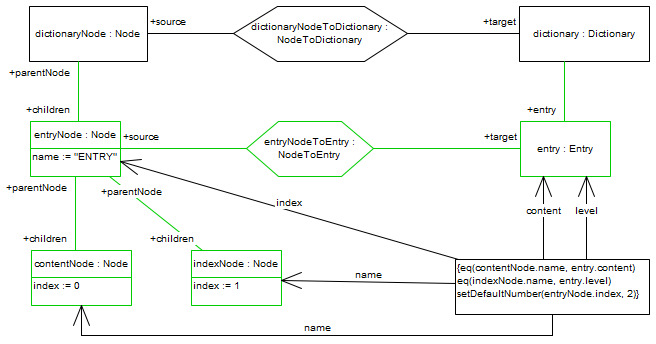
\includegraphics[width=\textwidth]{ea_ForAllEntryRule}
  \caption{completed ForAllEntry}
  \label{ea:ForAllEntry_Complete}
\end{center}
\end{figure}

\item[$\blacktriangleright$] Return to \texttt{NodeToDictionaryRule}. We need to think about what context elements we'll need for our next rule to handle
authors. Not only will we need \texttt{DictionaryNode} and \texttt{dictionary} as we did in \texttt{ForAllEntry}, we'll also need \texttt{shelf} and
\texttt{library} in order to satisfy the \texttt{Dictionary} metamodel, where each \texttt{author} is linked to both individual \texttt{dictionary} and
\texttt{library} elements. Derive and create \texttt{AuthorRule} as depicted below Fig.~\ref{ea:AuthorRule}

\begin{figure}[htbp]
\begin{center}
  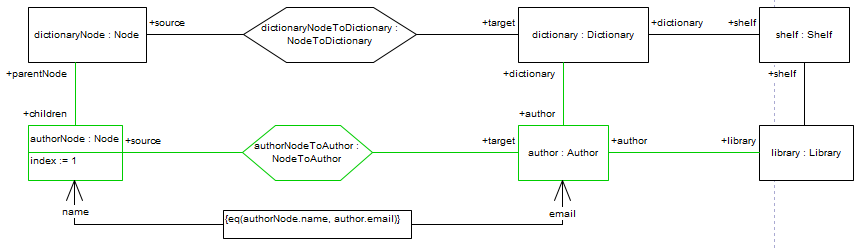
\includegraphics[width=\textwidth]{ea_AuthorRule}
  \caption{completed AuthorRule}
  \label{ea:AuthorRule}
\end{center}
\end{figure}

\item[$\blacktriangleright$] You're nearly done! Make sure everything is saved, and validate your TGG. If a dialogue appears saying the attempt was
unsuccessful, you may simply need to update your original schema diagram. To do so, open \texttt{dictionaryCodeAdapter}, right click anywhere in the diagram and
add any missing elements by navigating to ``Insert Existing Element'' (Fig.~\ref{ea:insertContext}), and selecting the missing correspondence types from the package's
tree (Fig.~\ref{ea:insertTree}).

\begin{figure}[htbp]
   \centering
      \subfloat[comment 1 \update]{
        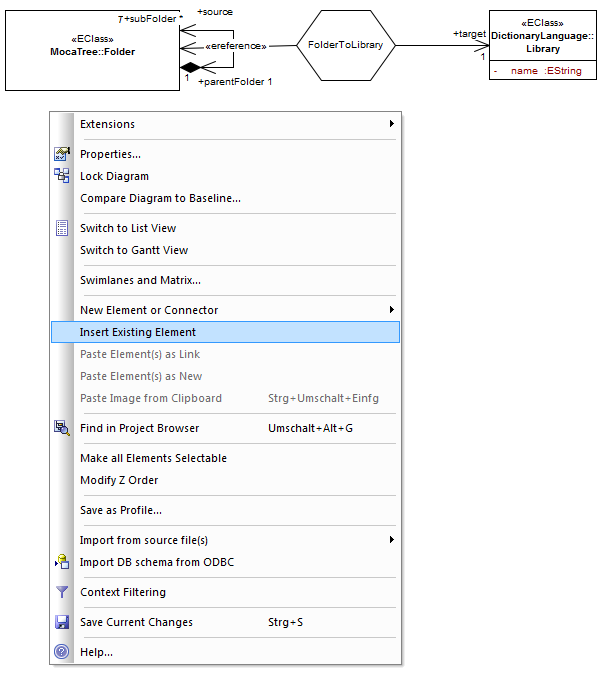
\includegraphics[width=0.45\textwidth]{ea_InsertExistingElements}
        \label{ea:insertContext}
      }
      \subfloat[Bugger. Comment 2]{
        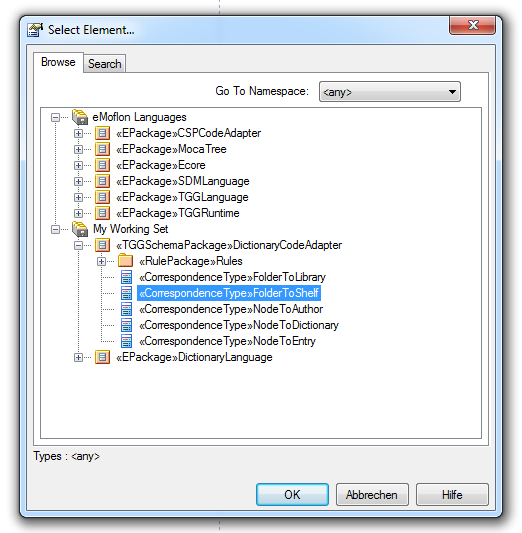
\includegraphics[width=0.45\textwidth]{ea_insertElementTree}
        \label{ea:insertTree}
      }
      \caption{Insert elements you created on the fly}
\end{figure}

\item[$\blacktriangleright$] Your schema diagram should come to resemble Fig.~\ref{ea:Schema_Complete}.

\begin{figure}[htbp]
\begin{center}
  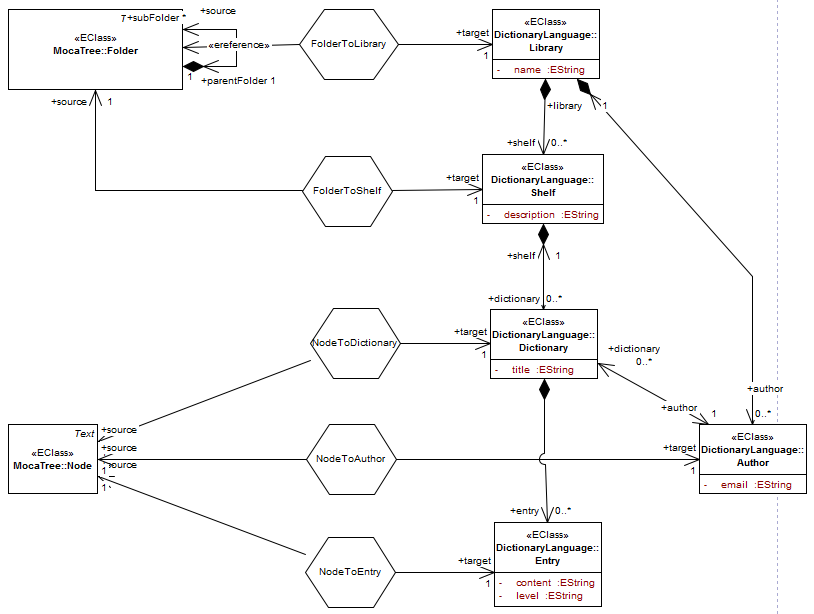
\includegraphics[width=\textwidth]{ea_finalSchema}
  \caption{completed Schema}
  \label{ea:Schema_Complete}
\end{center}
\end{figure}

Run TGG main -- two author nodes were created from
\texttt{numbers1-10.dictionary} and \texttt{numbers11-20.dictionary} having the same author. Having repeated, identical \texttt{author} elements may not always be desired. Wouldn't it sometimes be nice to have \emph{one} author can can be
connected to multiple \texttt{dictionary} elements?

\item[$\blacktriangleright$] We can use the basis of \texttt{AuthorRule} (return to this) for \texttt{ForAllNewAuthorRule} and \texttt{ExistingAuthorRule}. We
want to avoid copy and pasting where we can, but we need all the same elements. eMolfon's visual syntax has a cool \emph{refinement} feature, which enables you
to adjust only specific parts of an already created rule. First, return to the \texttt{Rules} diagram

\item[$\blacktriangleright$] Return to the main \texttt{Rules} diagram, and select \texttt{AuthorRule} and press \texttt{Alt + enter} to raise its properties
dialogue. Go to ``Properties/Details'' and select the \texttt{Abstract} box (Fig.~\ref{}).

\item[$\blacktriangleright$] Now create two new rules, \texttt{ForAllNewAuthorRule} and \texttt{ExistingAuthorRule}. Quick-link from each of them to
\texttt{AuthorRule} and select \texttt{Create Refinement Link}. Each of these now inherits the same pattern as \texttt{AuthorRule}.

\item[$\blacktriangleright$] Lets implement \texttt{ForAllNewAuthorRule}. Double-click its class and create a green \texttt{authorNode}, and black
\texttt{library} element. There's no need to worry about creating appropriate links; If you extend your imagination, picture this rule being placed on directly
on top of \texttt{AuthorRule}, like a clear cellophane sheet.\footnote{This may be easier to imagine if you place these objects in the same place as their
original}. While this rule doesn't actually modify anything from the original rule, this will make sense for the next rule.

\item[$\blacktriangleright$] Open the \texttt{ExistingAuthorRule} diagram. This time, we don't want to create an \texttt{authorNode}, but instead connect a
pre-existing \texttt{author} to \texttt{Library} (FIG). Compare this rule to its abstract.


\item[$\blacktriangleright$] Fantastic work: your forward transformation is now completed with TGGs. Try validating and exporting your package to Eclipse. If it
doesn't work at first, and everything has been done correctly, you may have to update the schema file -- it may be missing some elements you created on the fly.
Add any missing elements (it should resemble FIG), then validate again. Once it succeeds, refresh your Eclipse workspace to generate the corresponding code.


\jumpSingle{t2m close}

\end{itemize}


\newpage
\hypertarget{t2m close}{}
\subsection{Tree To Model Close}
\genHeader

\begin{itemize}

\item[$\blacktriangleright$] Navigate to ``src/org.moflon.tie'' right click and run TGGMain as application.

\begin{figure}[htbp]
\begin{center}
  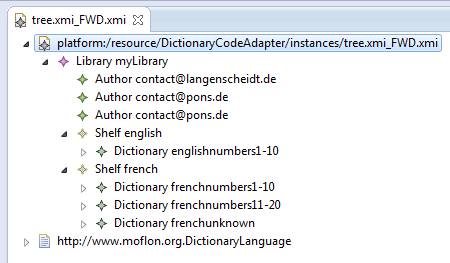
\includegraphics[width=0.7\textwidth]{eclipse_generatedForwardTransformation}
  \caption{completed forward transformation}
  \label{eclipse:generatedFwdTrsfm}
\end{center}
\end{figure}

\item[$\blacktriangleright$] Awesome, it works BEAUTIFULLY! Lets examine the output, \texttt{tree.xmi\_FWD.xmi} a little closer.

\item[$\blacktriangleright$] If you haven't already, read Section 6 from Part IV to learn how eMoflon's integrator feature can help you visualize how this
transformation was completed. Run the integrator on \texttt{corr\_FWD.xmi} until you reach the first (english) author node (do this as proof).

\begin{figure}[htbp]
\begin{center}
  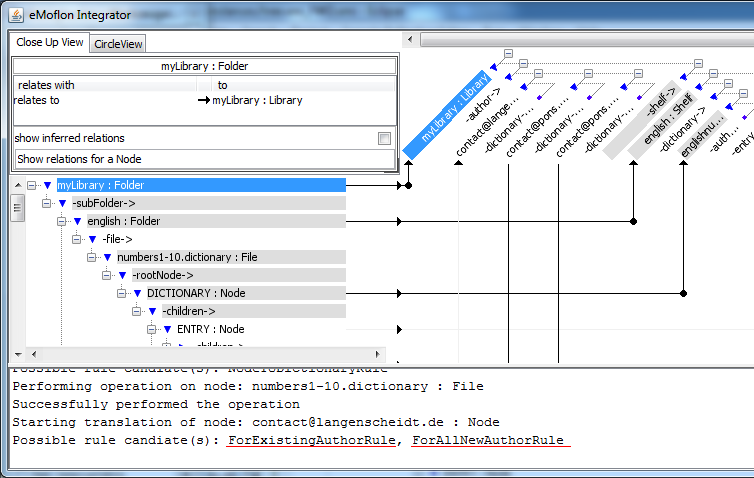
\includegraphics[width=0.7\textwidth]{eclipse_integratorAuthorChoice}
  \caption{completed forward transformation}
  \label{eclipse:generatedFwdTrsfm}
\end{center}
\end{figure}

\item[$\blacktriangleright$] The transformation decided to take one rule - either create or use existing - based on a random choice. The current set up isn't
dependable. We need to force a decision.

\item[$\blacktriangleright$] It had two choices and picked on at random. If you DO want to force a decision. You have two choices: ``I
don't care, \emph{always} make an author'' (duplicates), or no, ``I \emph{never} want there to be two of the same authors for one library.'' There are two ways
to define this: (Discuss options here?)

\end{itemize}

\begin{description}

\item[option1: Run-time] Create a configuration file for your TGG;

First: define \texttt{AuthorConfiguator}. FIG. put in in the same pacakage as your TGG. Don't make errors.

\begin{figure}[htbp]
\begin{center}
  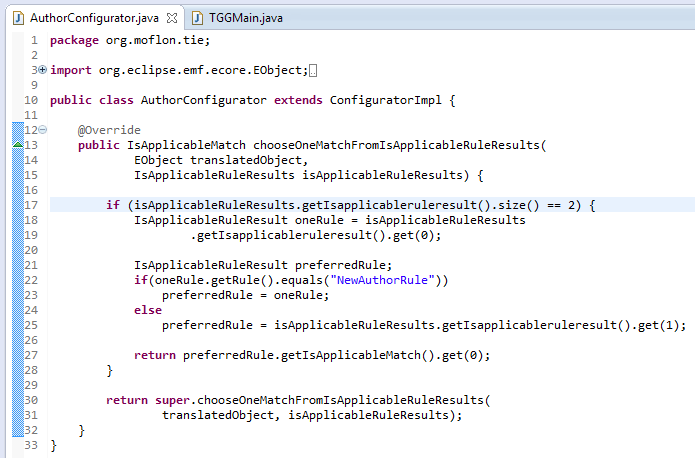
\includegraphics[width=0.7\textwidth]{eclipse_authorConfigurator}
  \caption{comment}
  \label{eclipse:authorConfig}
\end{center}
\end{figure}

Second: call it from \texttt{TGGMain}. FIG. Only need it in the forward transformation, so only put it once\ldots

\begin{figure}[htbp]
\begin{center}
  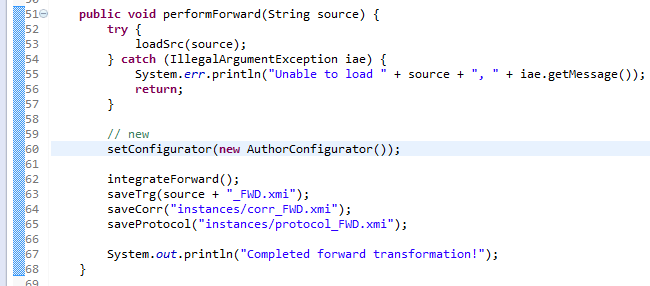
\includegraphics[width=0.7\textwidth]{eclipse_editTGGMain}
  \caption{comment on the edit}
  \label{eclipse:editTGGMain}
\end{center}
\end{figure}

\item[option2: Design-time] Create a NAC in \texttt{ForAllNewAuthors}; force it to skip
\hyperlink{NAC vis}{link1: {\bf VISUAL}}
\hyperlink{NAC tex}{link2: {\bf TEXTUAL}}

\input{../3_treeToModel/vis_designTimeNAC}

\input{../3_treeToModel/tex_designTimeNAC}

\end{description}

% Back together, run TGGMain again
\newpage
\begin{itemize}

\item[$\blacktriangleright$] With your forced set up now constructed, Run TGGMain again. Use the integrator once more to see how it consistently chose your
decision.

\item[$\blacktriangleright$] Great work! You have now completed the first half of the complete round trip transformation, from Text to Model!

\end{itemize}



% And back with TGGS
\newpage
\section{Model-To-Tree with TGGs}
\genHeader

One powerful benefit of working with TGG transformations is that by specifiying one transformation (i.e., a forward transformation), we're able to get the
opposite direction for free! Our example used a \texttt{tree.xmi} (\texttt{MocaTree}
instance) input, transformed it forward into \texttt{tree.xmi\_fwd.xmi} (\texttt{Dictionary} instance), and used that result file in a backwards
transformation to create the final tree output, \texttt{tree.xmi\_FWD.xmi\_BWD.xmi}, all without error! If our TGG was truly successful however,
the starting and final files should be identical. Let's compare the two (Fig.~\ref{eclipse:comparingTreeModels}).

\vspace{0.5cm}

\begin{figure}[htpb]
\begin{center}
  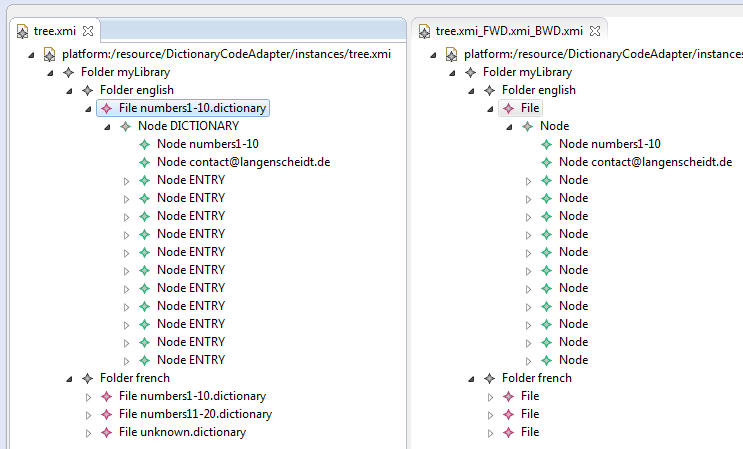
\includegraphics[width=\textwidth]{eclipse_generatedBackwardsModel}
  \caption{Not yet identical trees}
  \label{eclipse:comparingTreeModels}
\end{center}
\end{figure}

\vspace{0.5cm}

It's close, but not perfect. You can see that some things need to be refined. The ``DICTIONARY'' and ``ENTRY'' labels, for example, are missing from the
major nodes. We need to include an attribute constraint to bind these specific EString values. You'll also notice that, as you scroll through each
\texttt{Node}, the \texttt{title} and \texttt{author} nodes have the correct \texttt{index} values of 0 and 1, but the remaining \texttt{entry} indices are also
set to 0.
We were only concerned with binding the title and author nodes in the forward direction, as we could assume that any other node with any other index value (2 and greater) was an
\texttt{entryNode}. In the backwards direction however, this distinction is lost, which means we must introduce a custom attribute constraint.

\jumpDual{m2tvis}{m2ttex}

\newpage
\hypertarget{m2tvis}{}
\subsection{Double-checking the TGG}
\visHeader

\begin{itemize}

\item[$\blacktriangleright$] Open \texttt{NodeToDictionaryRule} and update as depicted below (via attribute constraint). Is this in the right place? Should this
be done before??

\begin{figure}[htp]
\begin{center}
  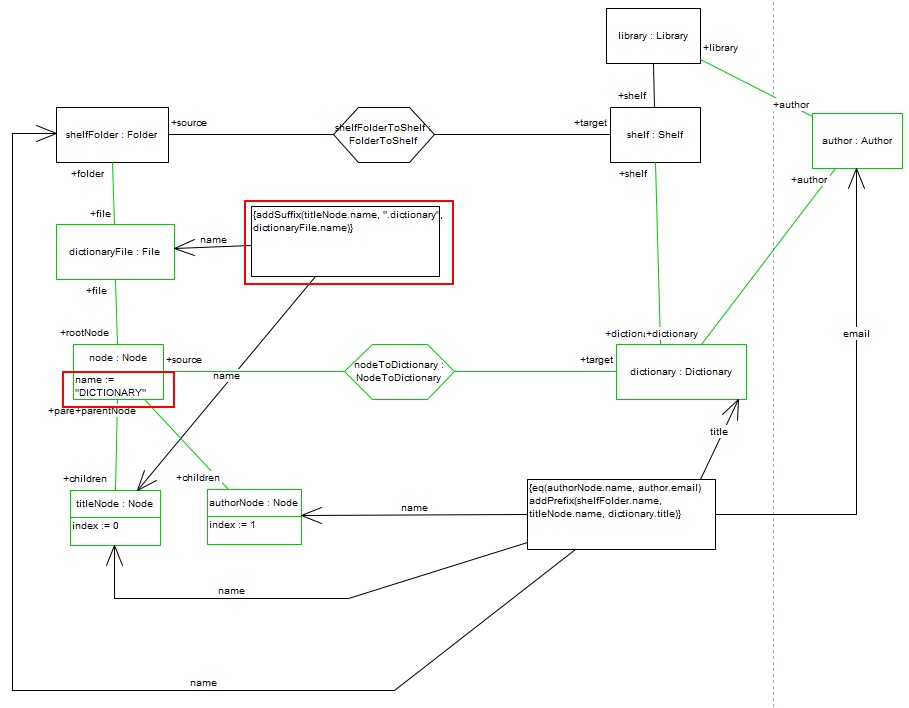
\includegraphics[width=\textwidth]{ea_updateNodeToDictionary}
  \caption{updated NodeToDictionary}
  \label{ea:NodeToDictionary_updated}
\end{center}
\end{figure}

\item[$\blacktriangleright$] Similarly, open \texttt{ForAllEntry} in EA and update like so:

\begin{figure}[htp]
\begin{center}
  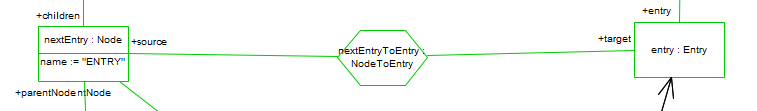
\includegraphics[width=\textwidth]{ea_updateForAllEntry}
  \caption{updated ForAllEntry}
  \label{ea:ForAllEntry_updated}
\end{center}
\end{figure}

\item[$\blacktriangleright$] End comment.

\jumpSingle{finalStep}

\end{itemize}


\newpage
\hypertarget{m2ttex}{}
\subsection{Refining the TGG Transformation}
\texHeader

\begin{itemize}

\item[$\blacktriangleright$] Find the relevant files and add the following attribute constraints. Note : the MOSL parser requires that all attribute constraints
are declared before link variables.

\begin{figure}[htp]
\begin{center}
  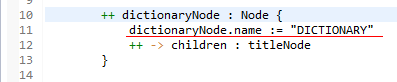
\includegraphics[width=0.8\textwidth]{eclipse_NodeToDictionaryRule_updated}
  \caption[labelInTOC]{needs refinement\ldots}
  \label{eclipse:generatedBkwrdMdl}
\end{center}
\end{figure}

\begin{figure}[htp]
\begin{center}
  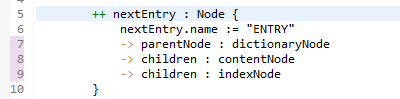
\includegraphics[width=0.8\textwidth]{eclipse_ForAllEntryRule_updated}
  \caption[labelInTOC]{needs refinement\ldots}
  \label{eclipse:generatedBkwrdMdl}
\end{center}
\end{figure} 

\item[$\blacktriangleright$] Add new SetDefaultNumber CSP here.

\begin{figure}[htbp]
\begin{center}
  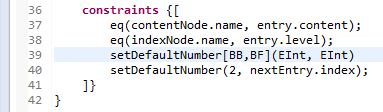
\includegraphics[width=0.6\textwidth]{eclipse_setDefaultNumberConstraint}
  \caption{extra constraint}
  \label{eclipse:newEntryConstraint}
\end{center}
\end{figure}

\end{itemize}


\newpage
\hypertarget{common cspConstraint}{}
\subsection{Implementing SetDefaultNumber}
\genHeader

We've declared and used our custom \texttt{SetDefaultNumber} constraint, but we haven't given it any implementation code yet. If you haven't yet, save and build
\texttt{DictionaryCodeAdapter} before continuing.

\begin{itemize}

\item[$\blacktriangleright$] Navigate to ``/src,'' where a new \texttt{csp.constraints} package was generated, and open \texttt{SetDefaultNumber.java}. Edit
this file until it matches Fig.~\ref{eclipse:setDefaultImpl}.

\begin{figure}[htbp]
\begin{center}
  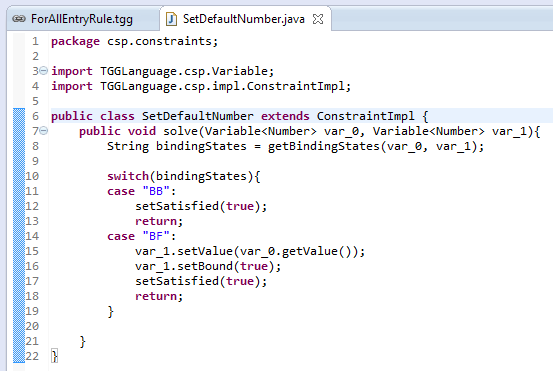
\includegraphics[width=0.9\textwidth]{eclipse_setDefaultNumberImplementation}
  \caption{extra constraint impl}
  \label{eclipse:setDefaultImpl}
\end{center}
\end{figure}

\item[$\blacktriangleright$] Save, build, and run \texttt{TGGMain} one more time. The inital and final \texttt{tree} variants should now be nearly identical! If
you're worried about some of the nodes being in the wrong order (such as an author at the bottom of the list), double-click on them and check their
\texttt{index} properties. If everything has been done correctly every \texttt{entry} should be 2, each \texttt{author} should be 1, and each \texttt{title}
should be 0.

\item[$\blacktriangleright$] On a final note to end the model-to-text step, wasn't it great how easy and short this was? If we were to use another
transformation set up (such as SDMs), we would have had to create independent rules for this backwards direction. Instead, TGGs gave us this transform for free!

\end{itemize}




\newpage
\hypertarget{finalStep}{}
\section{Tree-to-text transformation}
\genHeader

We've finally reached the last step, transforming our tree result, \texttt{fwd.trg.xmi} back into a filesystem with \texttt{.dictionary} files identical to our
original input, the \texttt{myLibrary} filesystem.

Note that in an actual application, we would do something useful with the model before transforming it back to text, or the dictionary might have been produced
from a learning box, i.e., the textual syntax representation wouldn't exist yet. One of the coolest things about ANTLR is that the same parsing technology that
we used in Section 2 can be used to \emph{unparse} the tree.

Analogously to parsing text with a lexer and parser grammar to produce a tree, a tree is unparsed to text using a \emph{tree grammar} and \emph{templates}. A
tree grammar is similar to EBNF, consisting of rules (\texttt{main}, \texttt{entry}) that each match a tree fragment and evaluate a template, as
opposed to rules that match text fragments and build a tree. For further details concerning tree grammars, we refer to \cite{ANTLR} and the ANTLR
website \url{www.antlr.org}.

\begin{itemize}

\item[$\blacktriangleright$] Expand ``src/org.moflon.moca.dictionary.unparser'', open \texttt{Dict\-ion\-ary\-Tree\-Gram\-mar.g}, and edit the contents as
depicted in Fig.~\ref{eclipse:treeGrammar}. 

\vspace{0.5cm}

\item[$\blacktriangleright$] Next, open \texttt{Dict\-ion\-ary\-Un\-pars\-er\-Ad\-ap\-ter.java} (Fig~\ref{eclipse:unparserCommented}). You'll notice that this
file contains a (commented) \texttt{StringTemplateGroup} meth\-od for retrieving a group of templates and needs to be implemented. The comments explain how to
use either a folder containing different template files, or a single file containing all templates. The latter is better for numerous small templates, while the
former makes sense when the templates contain a lot of static text.

\vspace{0.5cm}

\item[$\blacktriangleright$] For this small example, a single file with all templates is ideal. Uncomment line 44 (the option for a group file) and remove
the line throwing an \texttt{Un\-sup\-port\-ed\-Op\-er\-at\-ion\-Ex\-cep\-tion}.

\newpage 

\vspace*{2cm}

\begin{figure}[htpb]
\begin{center}
  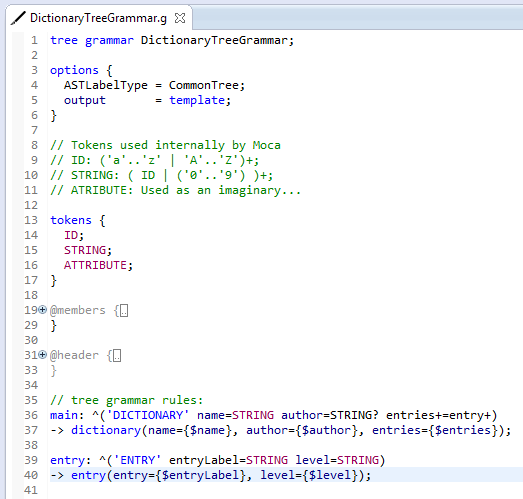
\includegraphics[width=0.8\textwidth]{eclipse_dictionaryTreeGrammar}
  \caption{Tree grammar for the unparser}
  \label{eclipse:treeGrammar}
\end{center}
\end{figure}

\vspace{1cm}

\begin{figure}[htpb]
\hspace{-1cm}
  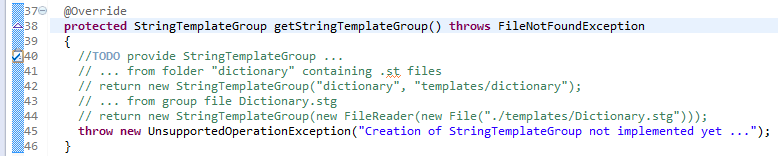
\includegraphics[width=1.2\textwidth]{eclipse_DictionaryUnparserAdapterUnimplemented}
  \caption{Two options of how to store templates}
  \label{eclipse:unparserCommented}
\end{figure}

\newpage


\item[$\blacktriangleright$] Create a template file by navigating to the empty ``templates'' folder of your adapter project, and creating a new file
named \texttt{Dictionary.stg} (as demanded in \texttt{Dict\-ion\-ary\-Un\-pars\-er\-Ad\-ap\-ter.java}). Complete it as specified in
Fig.~\ref{eclipse:dictionaryTemplate}.

\vspace{0.5cm}

\begin{figure}[htpb]
\begin{center}
  \includegraphics[width=0.5\textwidth]{eclipse_dictionaryTemplate}
  \caption{The \texttt{dictionary} template}
  \label{eclipse:dictionaryTemplate}
\end{center}
\end{figure}

\item[$\blacktriangleright$] Copy and paste \texttt{fwd.trg.xmi} into ``instances," naming the new file \texttt{bwd.src.xmi}. This will be the backward
transformation's input file.

\item[$\blacktriangleright$] Save and run your transformation again -- there should no longer be an error message in the console. Inspect and compare your input
and output folders and their containing files (Fig.~\ref{eclipse:unparseResult}). Are they the same?

\vspace{0.5cm}

\begin{figure}[htpb]
\begin{center}
  \includegraphics[width=0.4\textwidth]{eclipse_finalInstancesHierarchy}
  \caption{The final input and output filesystems}
  \label{eclipse:unparseResult}
\end{center}
\end{figure}

\item[$\blacktriangleright$] If everything succeeded, your transformation is now complete in both directions! Feel free to play around with
changing some files such as a the unparser template, or the content of the original files. How are the changes propagated through the transformation?
How about implementing an SDM to refactor or extend the library model in some useful way before transforming it to text?

\end{itemize}


% Conclusion to forward users onto other parts
\newpage
\section{Conclusion and next steps}
\genHeader

This is the end!


% -- References
\newpage \genHeader
\phantomsection
\addcontentsline{toc}{section}{References}
\renewcommand*{\bibname}{References}
\bibliographystyle{plain}  
\bibliography{../../06_miscellaneous/commonFiles/references}

% Glossary?
% \newpage
\phantomsection
\addcontentsline{toc}{section}{Glossary}

\vspace{1cm}
{\Huge \bf Glossary}
\vspace{1cm}

\begin{description}

\item[\bf Abstract Syntax] 
Defines the valid static structure of members of a language. 

\item[\bf Concrete Syntax]
How members of a language are represented. This is often done textually or visually.

\item[\bf Constraint Language] 
Typically used to specify complex constraints (as part of the static semantics of a language) that cannot be expressed in a metamodel.

\item[\bf Dynamic Semantics] 
Defines the dynamic behaviour for members of a language.

\item[\bf Grammar] 
A set of rules that can be used to generate a language. 

\item[\bf Graph Grammar] 
A grammar that describes a graph language. This can be used instead of a metamodel or type graph to define the abstract syntax of a language.

\item[\bf Meta-Language] 
A language that can be used to define another language.

\item[\bf Meta-metamodel] 
A \emph{modeling language} for specifying metamodels.

\item[\bf Metamodel] 
Defines the abstract syntax of a language including some aspects of the static semantics such as multiplicities. 

\item[\bf Model] 
Graphs which conform to some metamodel.

\item[\bf Modelling Language] 
Used to specify languages. Typically contains concepts such as classes and connections between classes.

\item[\bf Static Semantics] 
Constraints members of a language must obey in addition to being conform to the abstract syntax of the language.

\item[\bf Type Graph] 
The graph that defines all types and relations that form a language. Equivalent to a metamodel but without any static semantics.

\item[\bf Unification]  
An extension of the object oriented ``Everything is an object'' principle, where everything is regarded as a model, even the metamodel which defines other
models.

\end{description}


\end{document}